\documentclass[default,sn-basic]{sn-jnl}

\usepackage{graphicx}
\usepackage{multirow}
\usepackage{amsmath,amssymb,amsfonts}
\usepackage{amsthm}
\usepackage{mathrsfs}
\usepackage[title]{appendix}
\usepackage{xcolor}
\usepackage{textcomp}
\usepackage{manyfoot}
\usepackage{booktabs}
\usepackage{algorithm}
\usepackage{algorithmicx}
\usepackage{algpseudocode}
\usepackage{listings}
\usepackage{tabularx}
\usepackage{url}

\newcolumntype{Y}{>{\raggedright\arraybackslash\hyphenpenalty=50\exhyphenpenalty=50}X}

\jyear{2026}

\raggedbottom

\begin{document}

\title[Who Wanted What in Brazil's ``Citizen Constitution''?]{Who Wanted What in Brazil's ``Citizen Constitution''? Network Communities and Sociodemographic Cleavages in 72,719 Letters to the 1988 Constituent Assembly}

\author[1]{\fnm{Rafael} \sur{Roseira Machado}}\email{rafaelroseira@alunos.utfpr.edu.br}
\author*[1]{\fnm{Andr\'{e} Luiz Satoshi} \sur{Kawamoto}}\email{kawamoto@utfpr.edu.br}

\affil*[1]{\orgdiv{Department of Computer Science}, \orgname{Federal University of Technology -- Paran\'{a} (UTFPR)}, \orgaddress{\street{Via Rosalina Maria dos Santos, 1233}, \city{Campo Mour\~{a}o}, \postcode{87301-899}, \state{Paran\'{a}}, \country{Brazil}}}

\abstract{Between 1986 and 1987, during Brazil's democratic transition from military rule, the Federal Senate conducted one of the largest pre-Internet participatory democracy experiments: the Citizen Information Support System (SAIC). Across all 26 Brazilian federative units, 72,719 citizen letters containing constitutional proposals were digitized and indexed into 24 bureaucratic themes. While qualitative studies examined isolated subsets, the complete corpus has never been modeled simultaneously through complex networks and multi-dimensional sociodemographic stratification. We present an end-to-end Computational Social Science framework that: (i) audits the 72,719-record historical database, correcting 323 spreadsheet formula corruption artifacts (\texttt{\#NOME?}); (ii) constructs a Positive Pointwise Mutual Information (PPMI) word co-occurrence network over =70,151$ unique valid letters; (iii) extracts emergent discourse communities via Louvain modularity maximization; and (iv) cross-tabulates these bottom-up communities against the 1986 top-down taxonomy, six sociodemographic dimensions (gender, urban/rural residence, mobilization mode, age cohorts, education, and income), geographic units, and bipartite lawmaker targeting. Sensitivity analysis identifies an optimal connected network ($|V|=322$ nodes, $|E|=1,823$ edges, density .53\%$) with high modularity (=0.6363$) across eight cohesive thematic communities. The study is descriptive and exploratory, documenting how constitutional priorities were distributed across social groups within this historic self-selected participatory corpus without claiming causal identification or universal population representativeness. All curated datasets, code, and high-resolution visualization pipelines are made openly available.}

\keywords{Complex Networks, Community Detection, Pointwise Mutual Information, Computational Social Science, Participatory Democracy, 1988 Brazilian Constitution}

\maketitle

\section{Introduction}\label{sec1}
The drafting of the 1988 Brazilian Federal Constitution---widely known as the ``Citizen Constitution'' (\textit{Constitui\c{c}\~{a}o Cidad\~{a}})---marked the institutional culmination of Brazil's transition from a 21-year authoritarian military regime (1964--1985) to a pluralist democracy \citep{souza2008regras,mcdonald2022making}. Well before the advent of the commercial Internet and modern digital e-participation platforms \citep{stieglitz2013social,pogrebinschi2014impact}, the Brazilian Federal Senate's Data Processing Center (Prodasen) launched an unprecedented sociotechnical initiative between March 1986 and mid-1987: the Citizen Information Support System (\textit{Sistema de Apoio Inform\'{a}tico ao Cidad\~{a}o} -- SAIC), also known as ``Project Constitution'' (\textit{Projeto Constitui\c{c}\~{a}o}) \citep{mcdonald2022making,santos2024lazer}. Through millions of postage-paid forms distributed in post offices, schools, city councils, and labor unions nationwide, ordinary citizens were invited to write their demands for the new constitutional text and optionally address them to specific members of the National Constituent Assembly (\textit{Assembleia Nacional Constituinte} -- ANC) \citep{montambeault2018constituicao,mcdonald2022making}.

In total, 72,719 citizen letters were transcribed into Prodasen's mainframe database, recording not only the free-text constitutional suggestion (\texttt{TEXTO SUGEST\~{A}O}) and an official classification into 24 thematic categories (\texttt{CAT\'{A}LOGO}), but also a rich vector of self-reported sociodemographic and political attributes: gender (\texttt{SEXO}), age group (\texttt{FAIXA ET\'{A}RIA}), urban vs.\ rural residence (\texttt{MORADOR}), educational attainment (\texttt{INSTRU\c{C}\~{A}O}), occupation (\texttt{PROFISS\~{A}O}), family income bracket in minimum wages (\texttt{FAIXA RENDA}), state and municipality of origin (\texttt{UF}, \texttt{LOCALIDADE}), and the targeted parliamentarian (\texttt{DESTINAT\'{A}RIO}).

Despite its extraordinary value for Computational Social Science \citep{lazer2009computational,grimmer2013text}, prior scholarship on the SAIC database has suffered from two fundamental limitations. First, studies in political science and constitutional history have relied either on descriptive tallies of Prodasen's pre-assigned 24 bureaucratic categories or on qualitative reading of small topical samples \citep{mcdonald2022making,santos2024lazer}. Because the 24 official categories were designed \textit{a priori} by Senate information scientists in 1986 (a \textit{top-down} taxonomy), broad categories such as \textit{Social Organization} ($15,187$ occurrences) and \textit{Law -- State Organization} ($15,720$ occurrences) conflated vastly different grassroots grievances. Second, no prior peer-reviewed work has combined unsupervised \textit{bottom-up} semantic network modeling of the complete textual corpus with statistical stratification across the demographic, life-course, socioeconomic, geographic, and parliamentarian-targeting dimensions.

In this study, we bridge this gap by introducing an integrated Complex Network Analysis and Computational Social Science framework applied to the complete SAIC archive. % [NOVO] Escopo explícito
Our contribution is primarily \emph{descriptive and exploratory}: we aim to map how constitutional priorities were distributed across social groups and to what extent an unsupervised semantic partition recovers or disambiguates the official 1986 taxonomy, rather than to establish causal links between sociodemographic attributes and constitutional demands. Specifically, we address four research questions:
\begin{itemize}
    \item \textbf{RQ1 (Bottom-Up Semantic Structure):} What latent thematic communities emerge organically from the word co-occurrence network of the 70,151 unique constitutional proposals when weighted by Positive Pointwise Mutual Information (PPMI) and partitioned via Louvain modularity maximization?
    \item \textbf{RQ2 (Top-Down vs.\ Bottom-Up Alignment):} To what extent do the emergent network communities converge with or disambiguate the 24 official macro-themes indexed by Prodasen in 1986?
    \item \textbf{RQ3 (Sociodemographic, Mobilization \& Life-Course Cleavages):} How did constitutional priorities vary across gender, urban vs.\ rural residence, spontaneous vs.\ coordinated petition campaigns, life-course age cohorts, formal education, and income brackets?
    \item \textbf{RQ4 (Macro-Regional, State-Level \& Bipartite Parliamentarian Targeting):} How were grassroots demands and organized professional lobbying distributed across Brazil's macro-regions and states, and channeled toward specific Constituent Assembly leaders?
\end{itemize}

To ensure full reproducibility in accordance with Open Science principles, the curated dataset, high-resolution visualizations, and an interactive Google Colab replication notebook in English are publicly available at \url{https://github.com/alkawamo/snam-saic-1988} (and \url{https://github.com/alkawamo/base-saic}).

\section{Related Work}\label{sec2}
\subsection{Word Co-occurrence Networks and Community Detection in Political Texts}
Representing natural language corpora as complex networks---where vertices correspond to lexical units (lemmas) and edges capture statistically significant co-occurrence within a textual window or document---provides a transparent, mathematically grounded alternative to opaque neural representations, particularly in historical, clinical, and legal domains where lexical interpretability is paramount \citep{mota2012speech,amancio2015complex,quispe2021using,amancio2025leveraging}. However, raw co-occurrence counts in large corpora are heavily skewed by high-frequency general vocabulary, producing dense ``hairball'' topologies with poor modular discriminability \citep{turney2010frequency,quispe2021using}.

To overcome this bias, \citet{church1990word} introduced Pointwise Mutual Information (PMI), which measures how much the observed joint probability $P(w_i, w_j)$ exceeds the probability expected under statistical independence $P(w_i)P(w_j)$. Subsequent work demonstrated that truncating negative values to form Positive Pointwise Mutual Information (PPMI) \citep{bullinaria2007extracting,turney2010frequency}, combined with document-frequency filtering and percentile-based edge pruning, isolates genuine semantic associations and enables modularity-based community detection algorithms \citep{newman2006modularity,blondel2008fast,fortunato2010community,cordeiro2016dynamic,traag2019louvain} to recover coherent discourse frames in political corpora, legislative debates, and advocacy networks \citep{grimmer2013text,stieglitz2013social,rule2015lexical,bail2016combining}.

\subsection{Participatory Democracy and the 1988 Brazilian Constituent Assembly}
Historical and political science investigations of the 1988 Constituent Assembly have highlighted the dual nature of popular participation during Brazil's redemocratization \citep{souza2008regras,pogrebinschi2014impact,montambeault2018constituicao,mcdonald2022making}. While subsequent popular amendments (\textit{emendas populares}) required 30,000 signatures organized by civil society coalitions, the SAIC project (\textit{Projeto Constitui\c{c}\~{a}o}) represented an earlier, pre-constituent phase (1986--1987) open to any individual citizen \citep{mcdonald2022making,santos2024lazer}. \citet{mcdonald2022making} examined how ordinary citizens navigated these participatory channels during the democratic transition, while \citet{santos2024lazer} analyzed subsets of SAIC letters addressing leisure and social rights. Building upon these domain studies, the present work performs a rigorous programmatic audit of the complete 72,719-record dataset, establishes the quantitative correspondence between official top-down catalog themes and bottom-up network communities, and introduces a multi-dimensional stratification across demographic, socioeconomic, geographic, and parliamentary-targeting variables.

\section{Dataset Audit and Methodological Pipeline}\label{sec3}
\subsection{Methodological Framework}
Figure~\ref{fig:flowchart} outlines the end-to-end Computational Social Science framework employed in this study. The pipeline progresses through four distinct stages: (i) historical mainframe curation and data audit, correcting software-induced formula corruption; (ii) natural language preprocessing, vocabulary optimization, and Positive Pointwise Mutual Information (PPMI) network construction; (iii) unsupervised discourse community extraction via Louvain modularity maximization; and (iv) size-normalized projection onto individual letters followed by multi-dimensional demographic, life-course, geographic, and parliamentary stratification.

\begin{figure*}[t]
\centering
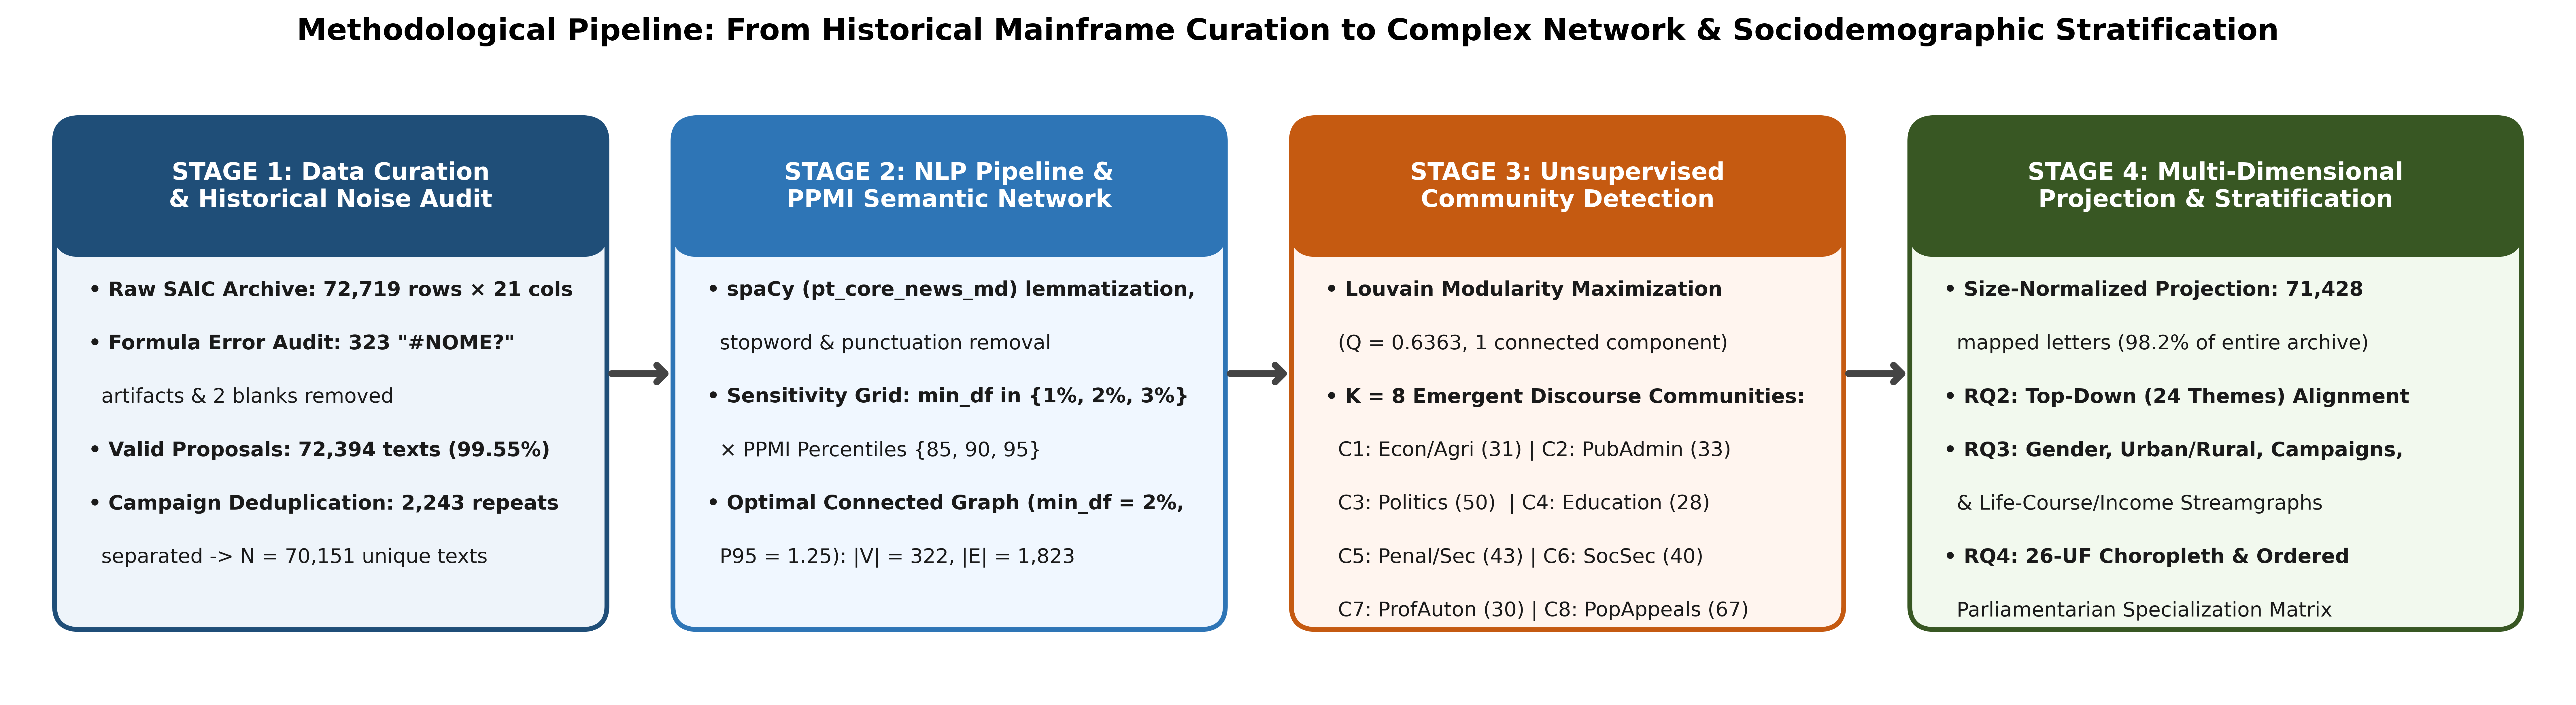
\includegraphics[width=\textwidth]{figures/fig0_pipeline_flowchart_en.png}
\caption{End-to-end methodological workflow: from historical data curation ($72,719$ raw records) and PPMI co-occurrence network formulation ($70,151$ unique texts) to Louvain community detection ($Q=0.6363$) and multi-dimensional sociodemographic projection ($71,428$ mapped letters).}
\label{fig:flowchart}
\end{figure*}

\subsection{Data Curation and Historical Noise Auditing}
The raw SAIC archive comprises $72,719$ rows and $21$ attributes. A comprehensive programmatic audit (summarized in Table~\ref{tab:audit}) revealed high completeness across core analytical variables, including $100\%$ coverage in state of origin (\texttt{UF}), municipality (\texttt{LOCALIDADE}), and official thematic catalog (\texttt{CAT\'{A}LOGO}), alongside $89.3\%$ to $94.7\%$ completeness in sociodemographic attributes (\texttt{SEXO}, \texttt{FAIXA ET\'{A}RIA}, \texttt{MORADOR}, \texttt{INSTRU\c{C}\~{A}O}, and \texttt{FAIXA RENDA}).

\begin{table}[t]
\caption{Audit of key attributes in the curated SAIC dataset ($72,719$ records).}\label{tab:audit}
\footnotesize
\setlength{\tabcolsep}{4pt}
\renewcommand{\arraystretch}{1.15}
\begin{tabularx}{\columnwidth}{@{}>{\raggedright\arraybackslash}p{2.6cm}rrY@{}}
\toprule
\textbf{Attribute} & \textbf{Missing} & \textbf{Valid (\%)} & \textbf{Description / Cardinality} \\
\midrule
\texttt{UF} / \texttt{LOCALIDADE} & 0 & 100.0\% & 26 States/\allowbreak Territories; 2,535 cities \\
\texttt{CAT\'{A}LOGO} & 0 & 100.0\% & 24 official Prodasen macro-themes \\
\texttt{TEXTO SUGEST\~{A}O} & 325 & 99.6\% & 72,394 valid; 70,151 unique texts \\
\texttt{FAIXA ET\'{A}RIA} & 4,756 & 93.5\% & 8 age cohorts (10--14 to $\ge 60$ yrs) \\
\texttt{SEXO} & 4,007 & 94.5\% & Male (45,356), Female (23,356) \\
\texttt{INSTRU\c{C}\~{A}O} & 4,734 & 93.5\% & 8 education levels (Illiterate to Postgrad.) \\
\texttt{MORADOR} & 6,257 & 91.4\% & Urban (58,950), Rural (7,512) \\
\texttt{FAIXA RENDA} & 7,774 & 89.3\% & 8 income brackets (No income to $>20$ MW) \\
\texttt{DESTINAT\'{A}RIO} & 48,187 & 33.7\% & 519 targeted Assembly members \\
\bottomrule
\end{tabularx}
\end{table}

Crucially, our inspection of \texttt{TEXTO SUGEST\~{A}O} uncovered a subtle data-corruption artifact: in addition to $2$ genuinely blank cells, exactly $323$ records contained the string \texttt{\#NOME?} (\texttt{\#NAME?}). Cross-checking these rows against historical metadata revealed that Prodasen typists frequently began itemized citizen letters with a hyphen or equals sign (e.g., \texttt{- Sugere que...}), which legacy spreadsheet software misinterpreted as invalid formula syntax during CSV export. Replacing these $323$ corrupted strings with null values yields $72,394$ valid natural-language texts. Furthermore, we identified $2,243$ duplicate submissions resulting from coordinated petition campaigns (such as standardized postcards distributed by schools, trade unions, and professional associations), leaving $N = 70,151$ unique valid texts.

\subsection{NLP Preprocessing and PPMI Network Formulation}
To prevent duplicate petition postcards from artificially distorting lexical co-occurrence probabilities, we construct the semantic network over the $N = 70,151$ unique texts and subsequently project all $72,719$ records onto the discovered communities. Each unique text was processed using the \texttt{pt\_core\_news\_md} pipeline in \texttt{spaCy}, retaining alphabetic tokens with length $>2$, removing standard Portuguese stopwords and punctuation, and reducing inflected forms to their canonical lemma. % [NOVO] Justificativa da coocorrência documental
Because citizen letters are short texts, we define co-occurrence at the document level rather than within sliding windows: a term pair is considered co-occurring when both lemmas appear in the same letter. This choice avoids the sparse-window problem typical of short documents and captures thematic association rather than local syntactic dependency.

Let $A \in \{0,1\}^{N \times |V|}$ denote the binary document--term incidence matrix over vocabulary $V$ constrained by a minimum document frequency threshold $\text{min\_df}$. The symmetric co-occurrence matrix is given by $C = A^{\top} A$ with $\text{diag}(C) = \mathbf{0}$. The empirical marginal probability of term $w_i$ is $P(w_i) = \text{diag}(A^{\top}A)_i / N$, and the joint document co-occurrence probability is $P(w_i, w_j) = C_{ij} / N$. We weight edges using Positive Pointwise Mutual Information (PPMI) \citep{church1990word,bullinaria2007extracting}:
\begin{equation}
    \text{PPMI}(w_i, w_j) = \max\left(0, \, \log_2 \frac{P(w_i, w_j)}{P(w_i)\,P(w_j)}\right).
\end{equation}
To prune spurious edges while maintaining global connectivity, we retain only edges $(w_i, w_j)$ whose weight satisfies $\text{PPMI}(w_i, w_j) \ge \theta_p$, where $\theta_p$ is the $p$-th percentile of all strictly positive PPMI values.

\subsection{Louvain Community Detection and Multi-Dimensional Stratification}
We partition the pruned weighted graph $G=(V,E,W)$ by maximizing Newman--Girvan modularity $Q$ \citep{newman2006modularity} via the Louvain algorithm \citep{blondel2008fast,cordeiro2016dynamic,traag2019louvain}:
\begin{equation}
    Q = \frac{1}{2m} \sum_{i,j \in V} \left[ W_{ij} - \frac{k_i k_j}{2m} \right] \delta(c_i, c_j),
\end{equation}
where $k_i = \sum_j W_{ij}$ is the weighted degree of node $i$, $m = \frac{1}{2}\sum_{i,j} W_{ij}$, and $\delta(c_i, c_j) = 1$ if nodes $i$ and $j$ belong to the same community $c \in \{C_1, \dots, C_K\}$.

Because communities vary in lexical size $|C_k|$, raw word counts favor larger communities. Therefore, for every citizen letter $d \in \{1, \dots, 72,719\}$ with binary lemma vector $\mathbf{x}_d \in \{0,1\}^{|V|}$, we define its size-normalized thematic affinity toward community $C_k$ as:
\begin{equation}
    s_{d,k} = \frac{\frac{1}{|C_k|} \sum_{w \in C_k} x_{d,w}}{\sum_{r=1}^{K} \frac{1}{|C_r|} \sum_{w \in C_r} x_{d,w}}, \quad \text{with } \sum_{k=1}^{K} s_{d,k} = 1.
\end{equation}
Out of all $72,719$ historical records, $71,428$ letters ($98.2\%$) contain at least one network lemma and thus possess a well-defined normalized thematic profile $\mathbf{s}_d = (s_{d,1}, \dots, s_{d,K})$ and dominant community $c^*(d) = \arg\max_k s_{d,k}$. % [ALTERADO] Distinção explícita entre as duas medidas
Two complementary measures are used throughout the paper and should not be conflated. First, the \emph{continuous thematic share} $s_{d,k}$ captures the full mixed profile of each letter; group-level averages $\bar{s}_{g,k}$ are the primary quantity reported in the streamgraphs and the grouped bar charts. Second, the \emph{dominant community} $c^*(d) = \arg\max_k s_{d,k}$ discretizes each letter into a single category and is used only to build the contingency tables underlying the Pearson Chi-square statistic $\chi^2$ and Cram\'{e}r's $V = \sqrt{\chi^2 / [n \min(R-1, K-1)]}$. The percentage-point differences reported in the text (e.g., $+9.1$ pp for women in $C_4$) are computed on the continuous shares $\bar{s}_{g,k}$, whereas the significance tests are computed on the dominant-community tables.

\section{Results and Discussion}\label{sec4}
\subsection{RQ1: Network Topology, Sensitivity Analysis, and Discourse Communities}
Table~\ref{tab:sensitivity} reports the topological and modularity metrics across nine combinations of $\text{min\_df} \in \{1.0\%, 2.0\%, 3.0\%\}$ and PPMI percentile cutoffs $p \in \{85, 90, 95\}$. At lower pruning thresholds ($p=85$ or $90$), excessive inter-topic edges limit modularity ($Q \in [0.39, 0.54]$). At $p=95$, $\text{min\_df}=1.0\%$ yields high modularity ($Q=0.5877$) but fragments the graph into $2$ components, whereas $\text{min\_df}=3.0\%$ severely restricts the vocabulary ($|V|=171$) and fractures the network into $3$ disconnected components. The intermediate parameterization---\textbf{$\text{min\_df}=2.0\%$ ($\ge 1,403$ unique letters) with the 95th percentile PPMI cutoff ($\theta_{95}=1.25$)}---uniquely preserves a single connected component ($1$ component, $|V|=322$ nodes, $|E|=1,823$ edges, density $3.53\%$) while achieving the global maximum modularity of \textbf{$Q = 0.6363$} across $K=8$ communities.

\begin{table*}[t]
\caption{Sensitivity analysis of document frequency ($\text{min\_df}$) and PPMI percentile pruning ($p$).}\label{tab:sensitivity}
\centering
\footnotesize
\setlength{\tabcolsep}{8pt}
\renewcommand{\arraystretch}{1.15}
\begin{tabular}{@{}lcccccccc@{}}
\toprule
\textbf{min\_df} & \textbf{Perc.} & $\boldsymbol{\theta_p}$ & $\boldsymbol{|E|}$ & $\boldsymbol{|V|}$ & \textbf{Dens.} & \textbf{Comp.} & $\boldsymbol{Q}$ & $\boldsymbol{K}$ \\
\midrule
1.0\% & 85 & 0.72 & 34,296 & 723 & 13.14\% & 1 & 0.3936 & 6 \\
1.0\% & 90 & 0.96 & 22,864 & 723 & 8.76\%  & 1 & 0.4676 & 6 \\
1.0\% & 95 & 1.38 & 11,432 & 715 & 4.48\%  & 2 & 0.5877 & 7 \\
\midrule
2.0\% & 85 & 0.65 & 5,467 & 322 & 10.58\% & 1 & 0.4535 & 6 \\
2.0\% & 90 & 0.88 & 3,645 & 322 & 7.05\%  & 1 & 0.5305 & 8 \\
\textbf{2.0\%} & \textbf{95} & \textbf{1.25} & \textbf{1,823} & \textbf{322} & \textbf{3.53\%} & \textbf{1} & \textbf{0.6363} & \textbf{8} \\
\midrule
3.0\% & 85 & 0.61 & 1,688 & 180 & 10.48\% & 1 & 0.4648 & 7 \\
3.0\% & 90 & 0.83 & 1,126 & 179 & 7.07\%  & 1 & 0.5432 & 6 \\
3.0\% & 95 & 1.19 & 563 & 171 & 3.87\%  & 3 & 0.6348 & 9 \\
\bottomrule
\end{tabular}
\end{table*}

Figure~\ref{fig:network} visualizes the optimal co-occurrence network ($|V|=322, |E|=1,823, Q=0.6363$) formatted with community separation halos and light inter-community edges, while Table~\ref{tab:communities} details the size, central nodes (degree, betweenness, and closeness within each induced community subgraph), and lexical profile of the eight emergent communities ($C_1$--$C_8$). Together, these communities span macroeconomic and agrarian policy ($C_1$), civil service and administrative structure ($C_2$), electoral rules and parliamentary mandates ($C_3$), public and religious education ($C_4$), criminal law, violence, and bioethics ($C_5$), retirement and healthcare ($C_6$), professional regulation and labor autonomy ($C_7$), and colloquial popular grievances against inflation, poverty, and the Jos\'{e} Sarney administration ($C_8$). % [NOVO] Problematização de C8
We note that $C_8$ is the most heterogeneous community in the network ($|C_8|=67$ lemmas, roughly twice the median community size). Its lexical profile mixes substantive grievances (poverty, hunger, corruption, the Sarney administration) with religious references (\textit{deus}) and epistolary formulas (\textit{carta, esperar}). Part of the signal captured by $C_8$ is therefore stylistic rather than strictly thematic: it aggregates the rhetorical register of ordinary citizens who wrote in a supplicant voice, rather than a single coherent policy domain. We retain $C_8$ because it is a robust and interpretable cluster at the chosen parameterization, but we interpret its substantive content with this caveat in mind.

\begin{figure*}[t]
\centering
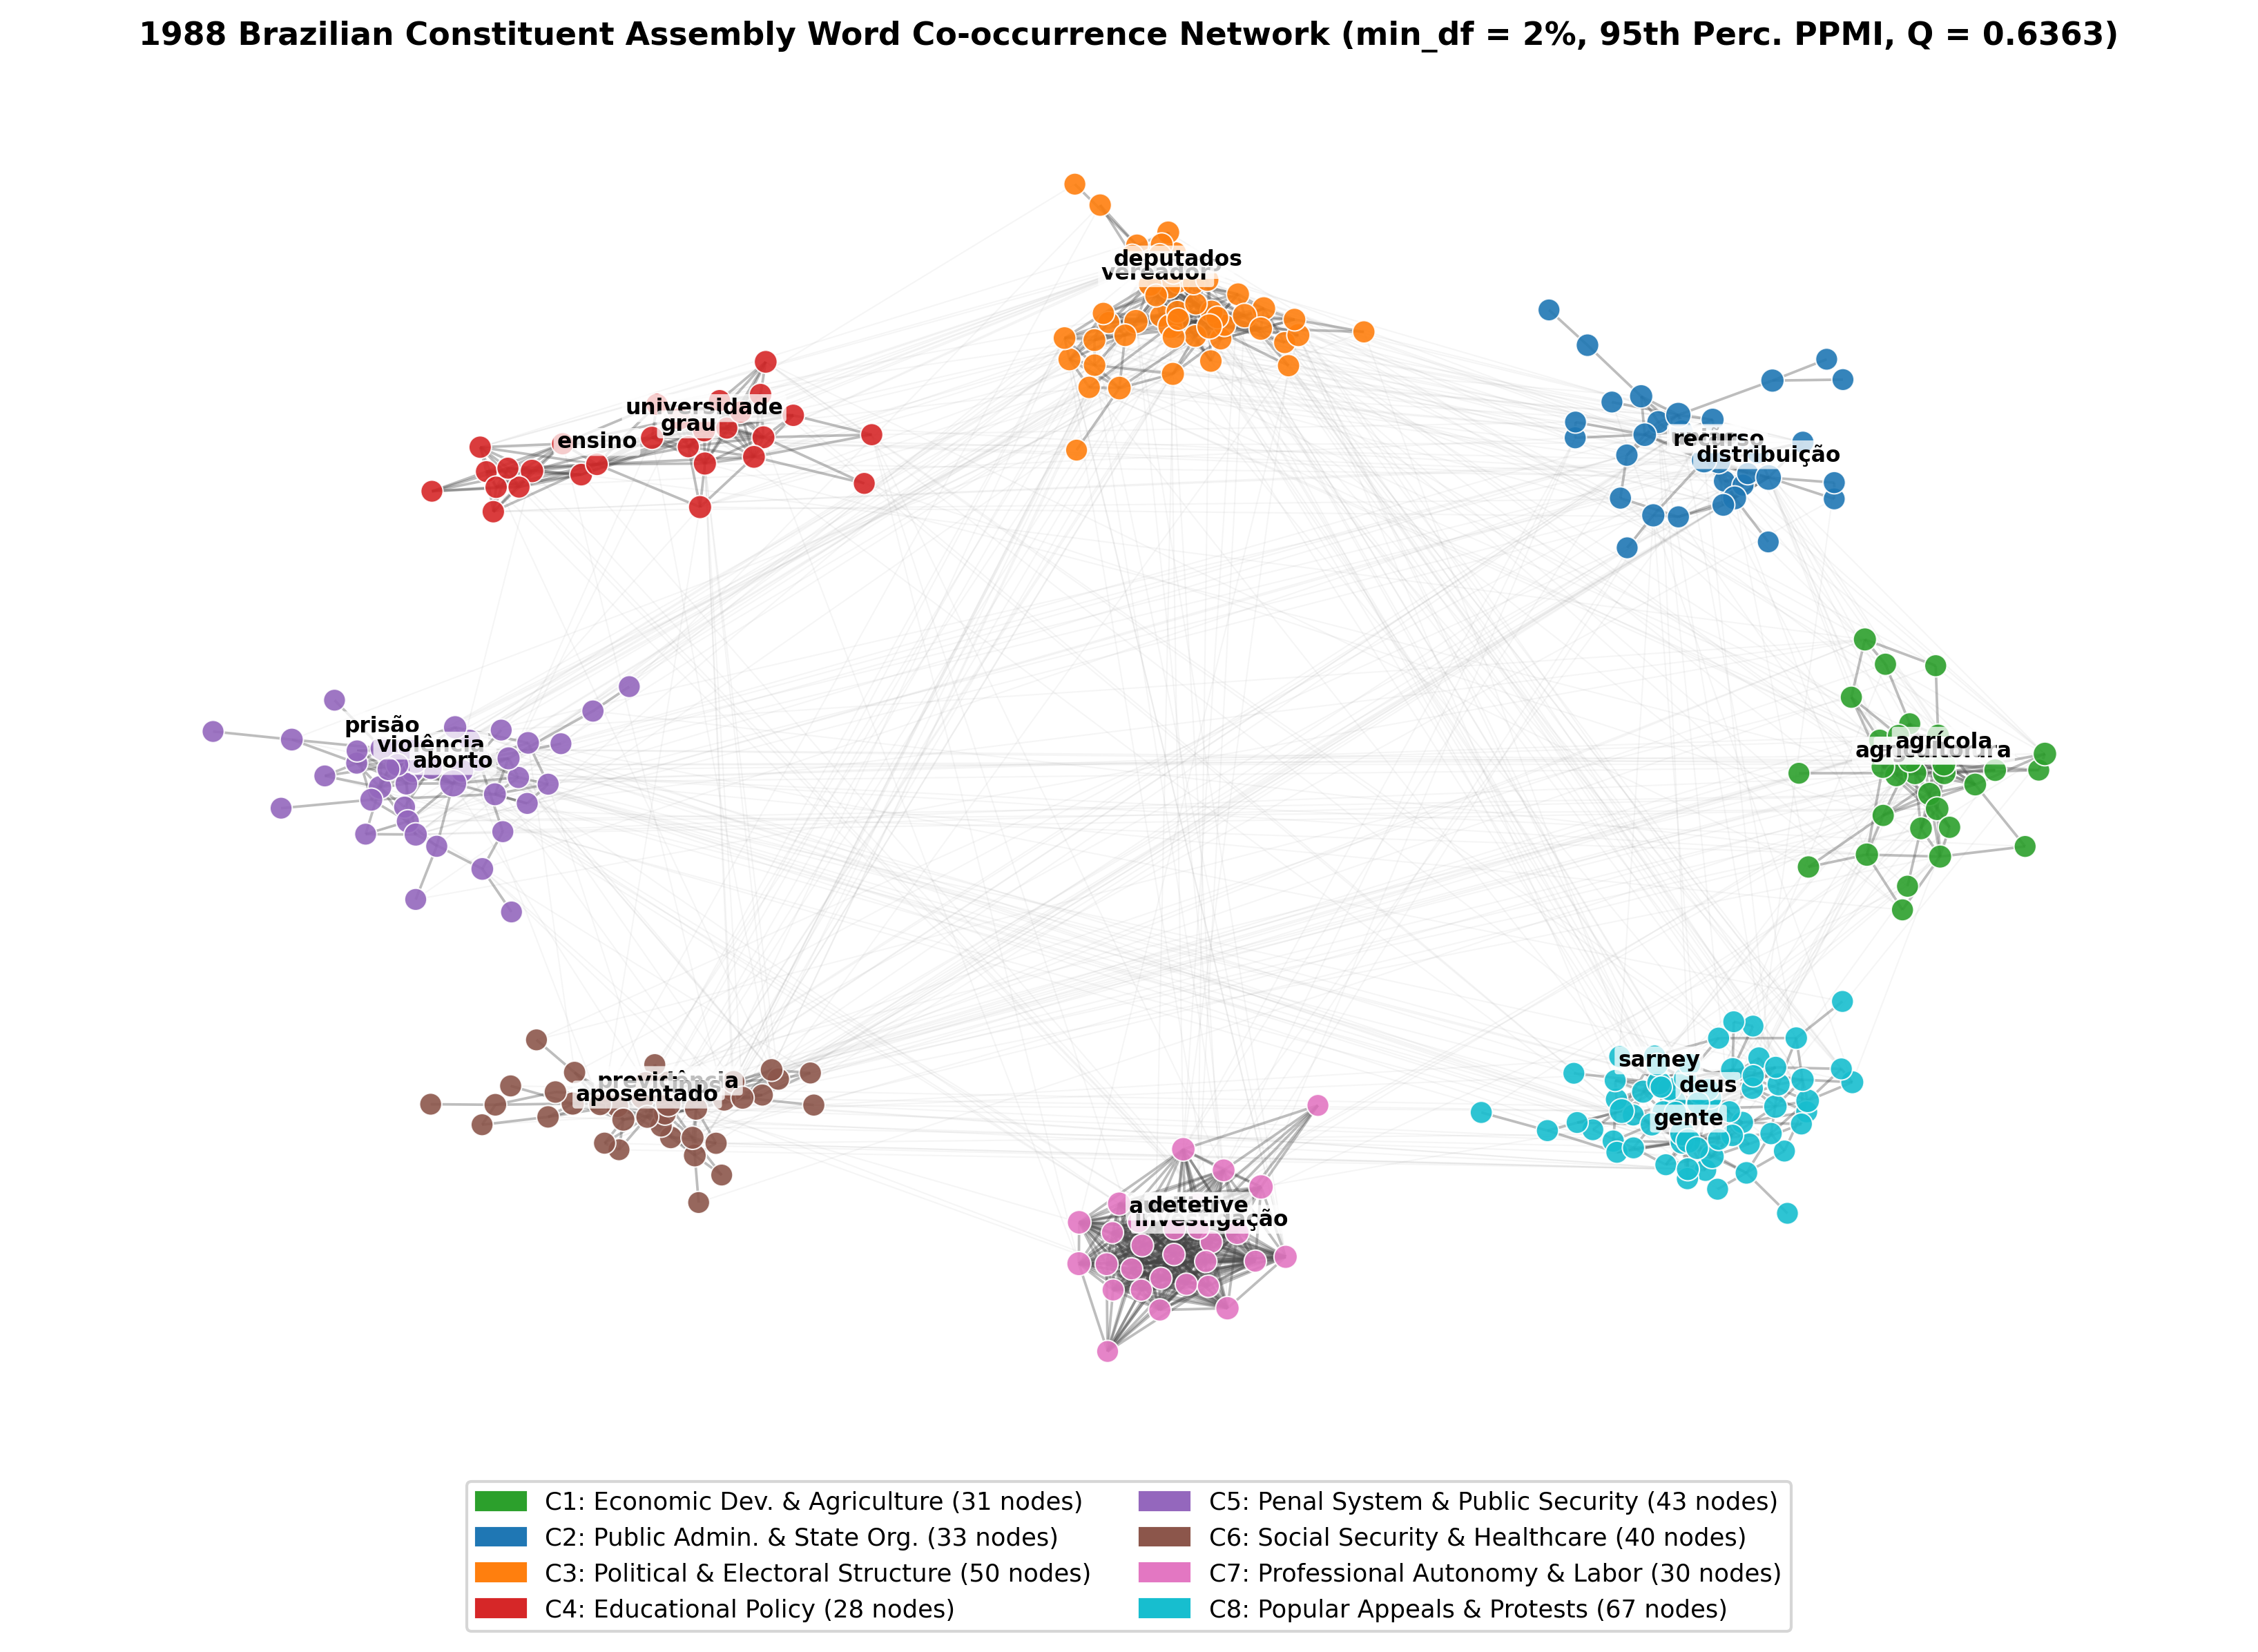
\includegraphics[width=\textwidth]{figures/fig1_cooccurrence_network_en.png}
\caption{Word co-occurrence network of the 1988 Brazilian Constituent Assembly ($\text{min\_df}=2.0\%$, 95th percentile PPMI cutoff $\theta_{95}=1.25$, $|V|=322$ nodes, $|E|=1,823$ edges, modularity $Q=0.6363$). Node colors indicate the 8 Louvain communities ($C_1$--$C_8$) and node sizes are proportional to global betweenness centrality. Inter-community edges are rendered with light opacity ($\alpha=0.022$) to ensure structural layering and separation.}
\label{fig:network}
\end{figure*}


\begin{table*}[t]
\caption{Characterization and intra-community centralities of the 8 Louvain discourse communities ($\text{min\_df}=2.0\%$, 95th percentile PPMI).}\label{tab:communities}
\footnotesize
\setlength{\tabcolsep}{5pt}
\renewcommand{\arraystretch}{1.25}
\begin{tabularx}{\textwidth}{@{}>{\raggedright\arraybackslash}p{3.6cm} c >{\raggedright\arraybackslash}p{2.3cm} >{\raggedright\arraybackslash}p{2.3cm} >{\raggedright\arraybackslash}p{2.3cm} X@{}}
\toprule
\textbf{ID \& Community Label} & $\boldsymbol{|C_k|}$ & \textbf{Max Degree} & \textbf{Max Betweenness} & \textbf{Max Closeness} & \textbf{Representative Lemmas (Portuguese)} \\
\midrule
\textbf{C1:} Economic Dev.\ \& Agriculture & 31 & \texttt{agricultura} (0.60) & \texttt{agricultura} (0.16) & \texttt{agricultura} (0.68) & \textit{agricultura, agr\'{\i}cola, terra, produzir, reforma, rural, banco, juro, d\'{\i}vida} \\
\textbf{C2:} Public Admin.\ \& State Org. & 33 & \texttt{uni\~{a}o} (0.41) & \texttt{uni\~{a}o} (0.38) & \texttt{uni\~{a}o} (0.56) & \textit{uni\~{a}o, estado, munic\'{\i}pio, imposto, tributo, recurso, distribui\c{c}\~{a}o, cargo, concurso} \\
\textbf{C3:} Political \& Electoral Structure & 50 & \texttt{mandato} (0.51) & \texttt{congresso} (0.13) & \texttt{mandato} (0.65) & \textit{congresso, deputado, senador, vereador, mandato, voto, elei\c{c}\~{a}o, partido, presidente} \\
\textbf{C4:} Educational Policy & 28 & \texttt{ensino} (0.56) & \texttt{ensino} (0.24) & \texttt{ensino} (0.69) & \textit{educa\c{c}\~{a}o, ensino, escola, universidade, curso, professor, aluno, gratuito, verba} \\
\textbf{C5:} Penal System \& Public Security & 43 & \texttt{pris\~{a}o} (0.36) & \texttt{aborto} (0.22) & \texttt{viol\^{e}ncia} (0.54) & \textit{crime, pena, morte, pris\~{a}o, viol\^{e}ncia, pol\'{\i}cia, menor, aborto, fam\'{\i}lia, moral} \\
\textbf{C6:} Social Security \& Healthcare & 40 & \texttt{previd\^{e}ncia} (0.41) & \texttt{previd\^{e}ncia} (0.26) & \texttt{previd\^{e}ncia} (0.58) & \textit{previd\^{e}ncia, inps, aposentadoria, aposentado, pens\~{a}o, sa\'{u}de, hospital, m\'{e}dico, idoso} \\
\textbf{C7:} Professional Autonomy \& Labor & 30 & \texttt{investiga\c{c}\~{a}o} (1.00) & \texttt{investiga\c{c}\~{a}o} (0.02) & \texttt{investiga\c{c}\~{a}o} (1.00) & \textit{detetive, investiga\c{c}\~{a}o, autonomia, aut\^{o}nomo, liberal, conselho, jornada, turno, hora} \\
\textbf{C8:} Popular Appeals \& Protests & 67 & \texttt{deus} (0.33) & \texttt{deus} (0.21) & \texttt{deus} (0.54) & \textit{povo, gente, pobre, fome, sofrer, deus, sarney, pol\'{\i}tico, corrup\c{c}\~{a}o, carta, esperar} \\
\bottomrule
\end{tabularx}
\end{table*}

\subsection{RQ2: Top-Down Official Taxonomy vs.\ Bottom-Up Semantic Communities}
Figure~\ref{fig:heatmap} presents the normalized cross-tabulation between Prodasen's 24 official catalog themes (\texttt{CAT\'{A}LOGO}) and the 8 network communities, rendered in the perceptually uniform and colorblind-safe \textit{viridis} palette. Several critical insights emerge:
\begin{enumerate}
    \item \textbf{Strong Diagonal Validation in Specialized Domains:} Where Prodasen's taxonomy was sectorally specific, the unsupervised PPMI+Louvain network recovers the exact institutional domain: \textit{Educational Policy} maps predominantly to $C_4$ ($34.8\%$), \textit{Agricultural Policy} ($26.6\%$) and \textit{Industrial Policy} ($21.0\%$) map to $C_1$, \textit{Social Security Policy} maps to $C_6$ ($26.1\%$), \textit{Politics -- State Structure} maps to $C_3$ ($21.3\%$), and \textit{Public Manifestation/Protest} ($27.0\%$) and \textit{Constituent Information Request} ($33.6\%$) map to $C_8$.
    \item \textbf{Disambiguation of Bureaucratic Catch-All Categories:} The two largest official themes---\textit{Law -- State Organization} ($15,720$ records) and \textit{Social Organization} ($15,187$ records)---are decomposed by the network primarily into $C_5$ (Penal System, Public Security \& Family/Bioethics: $18.8\%$ and $17.8\%$), $C_2$ (Public Administration: $14.6\%$ and $13.0\%$), and $C_6$ (Social Security \& Healthcare: $12.8\%$ and $14.0\%$), exposing the punitive and moral debates (e.g., capital punishment, criminal age of majority, abortion) that were obscured under generic legal headings.
    \item \textbf{Discovery of Coordinated Corporatist Mobilization in Labor Policy:} Letters indexed under \textit{Labor Policy} ($11,833$ records) split sharply between $C_6$ ($18.7\%$: retirement and welfare benefits) and $C_7$ ($17.1\%$: professional regulation and autonomous workers), reflecting the massive postal campaign waged by private detectives and liberal professionals demanding constitutional recognition.
    % [NOVO] Comparação equilibrada: o que a rede funde
    \item \textbf{The Network Also Merges Official Categories:} The bottom-up partition is not strictly finer than the 1986 taxonomy. Because the network has eight communities against 24 official themes, some administratively distinct categories are necessarily folded together. For instance, \textit{Agricultural Policy} and \textit{Industrial Policy} both concentrate in $C_1$ ($26.6\%$ and $21.0\%$), and \textit{Public Manifestation/Protest} and \textit{Constituent Information Request} both concentrate in $C_8$ ($27.0\%$ and $33.6\%$). The value of the network partition therefore lies in \emph{disambiguating catch-all categories and exposing cross-cutting substantive debates}, not in uniformly outperforming the official taxonomy on every dimension; for sectorally specific themes, the two partitions largely agree.
\end{enumerate}

\begin{figure*}[t]
\centering
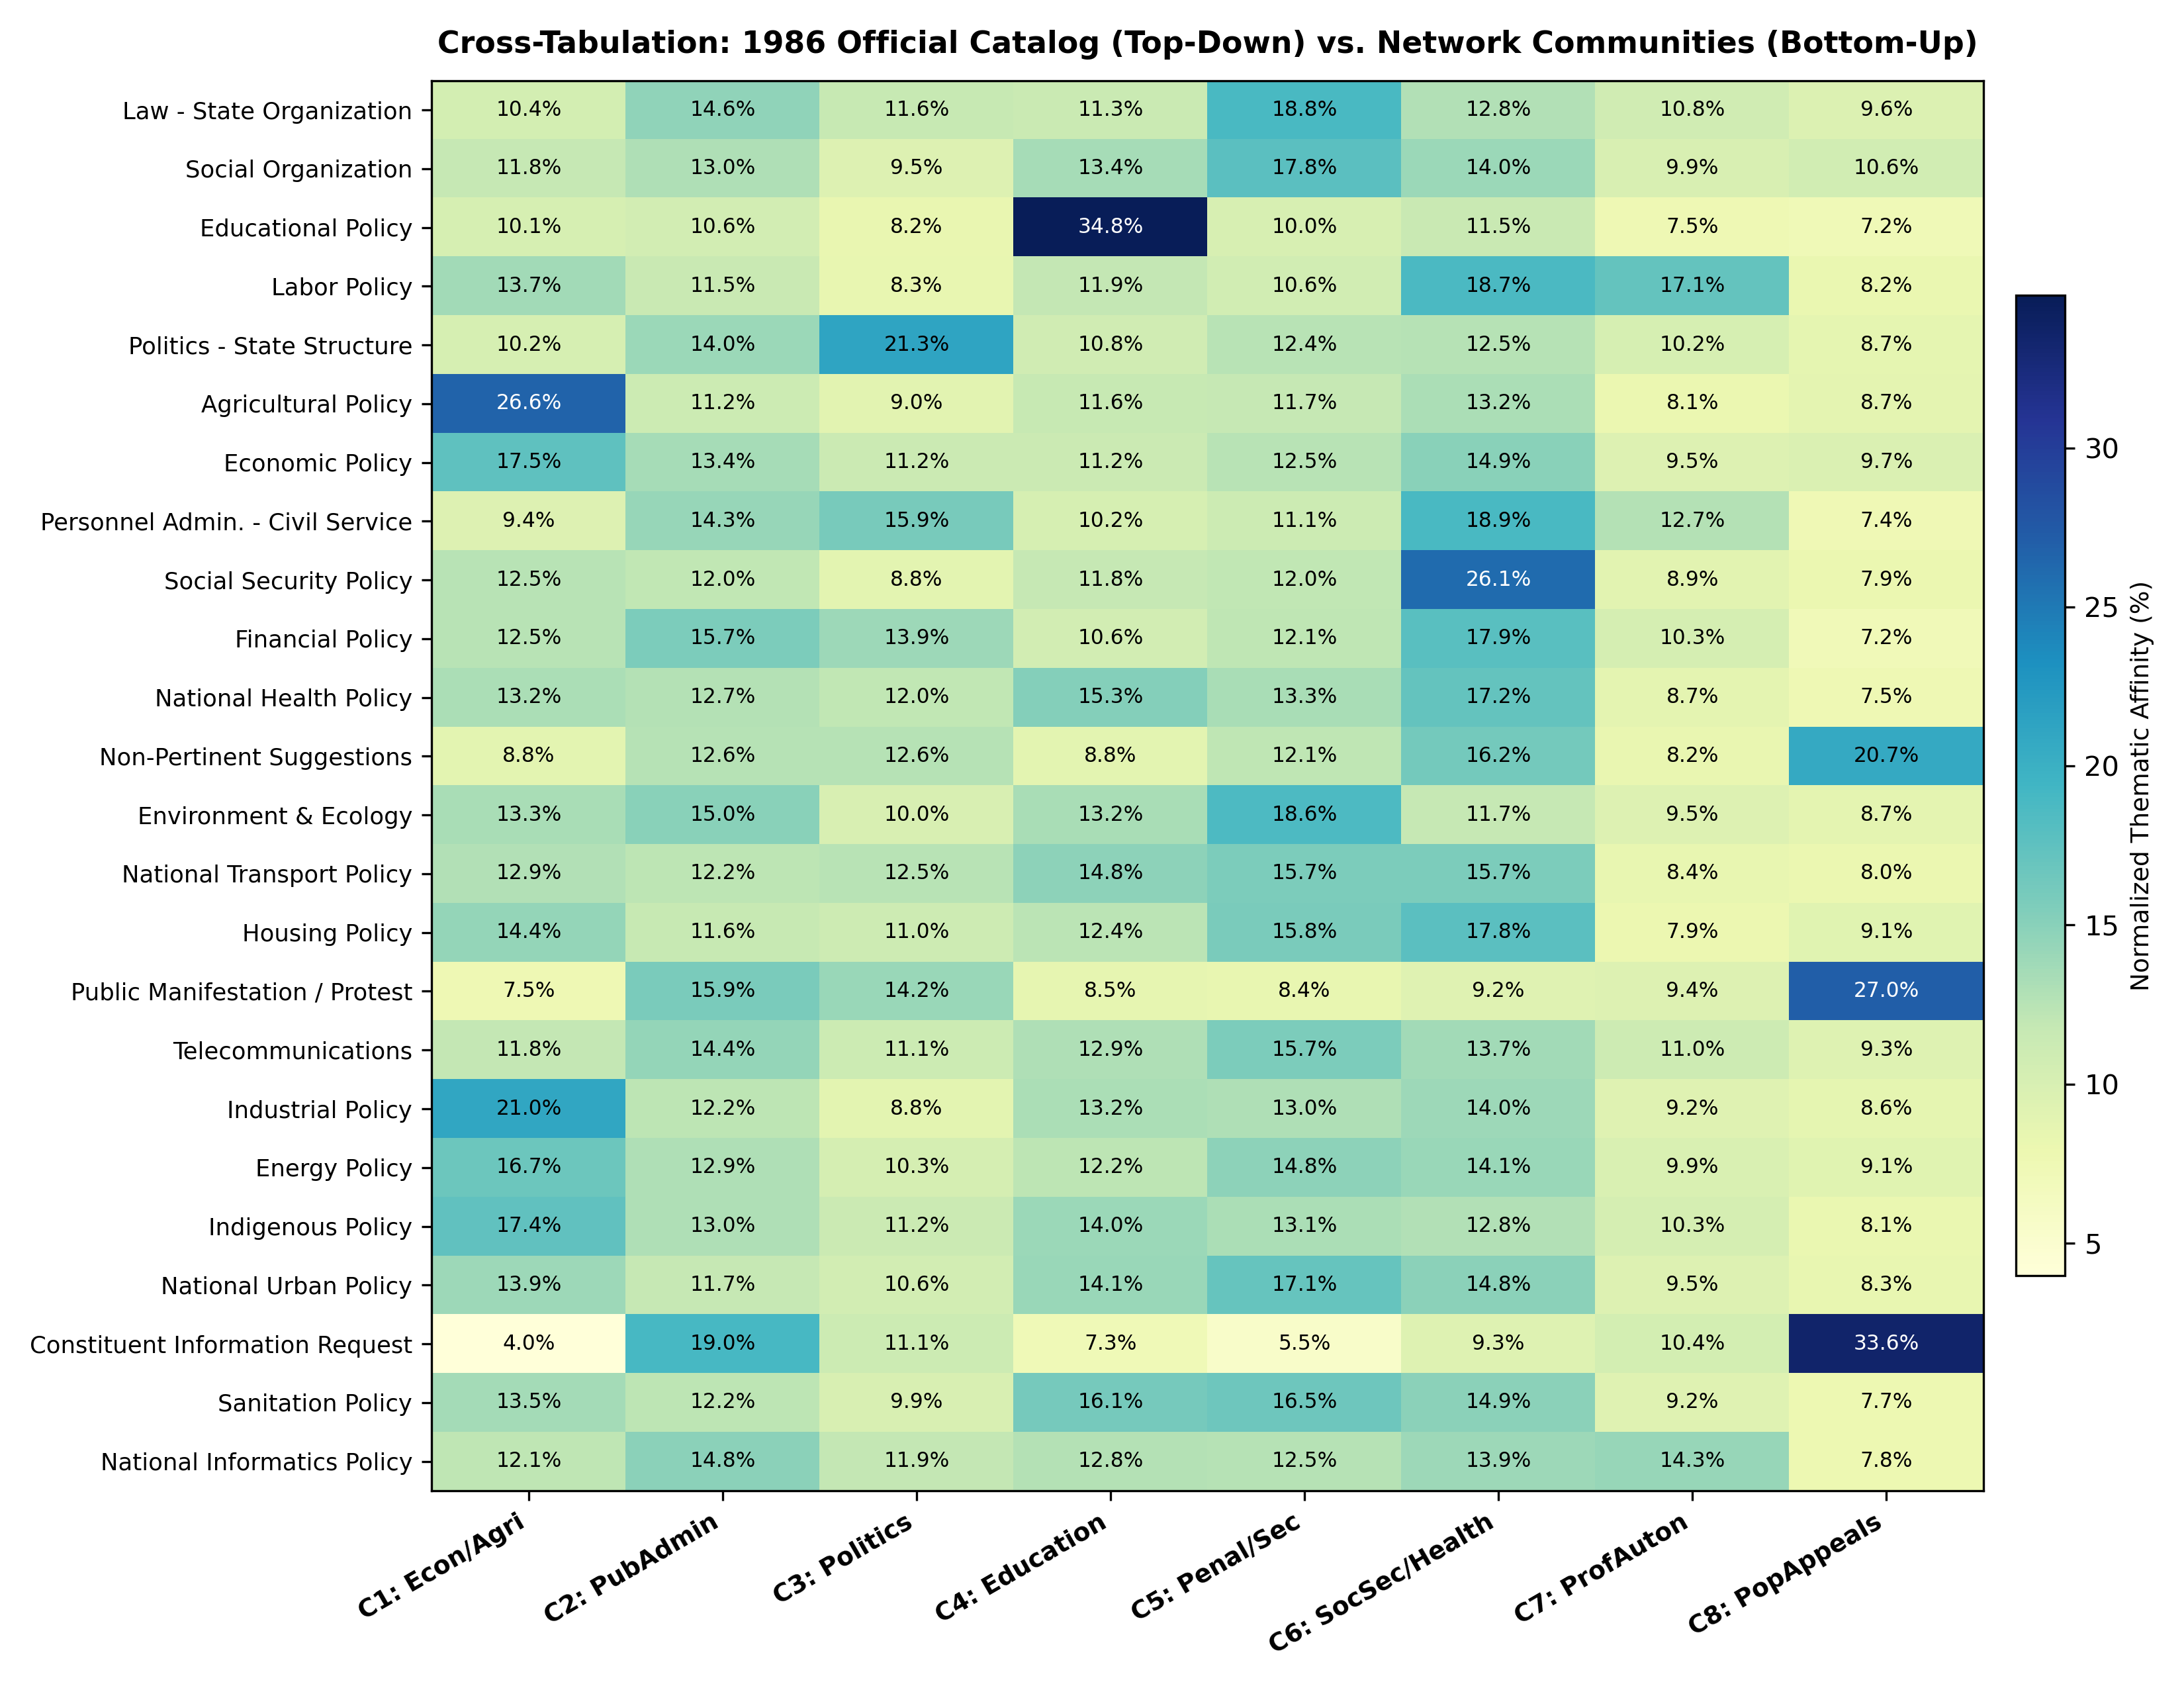
\includegraphics[width=\textwidth]{figures/fig2_topdown_vs_bottomup_heatmap_en.png}
\caption{Normalized contingency heatmap (\%) comparing the 24 official Prodasen macro-themes (\textit{top-down} classification, rows) against the 8 Louvain network communities (\textit{bottom-up} semantic extraction, columns) across $71,428$ citizen letters, rendered in the colorblind-safe \textit{viridis} colormap.}
\label{fig:heatmap}
\end{figure*}

\subsection{RQ3: Sociodemographic Cleavages, Mobilization Modes, and Life-Course Streamgraphs}
Figure~\ref{fig:demographics} pairs grouped thematic shares with diverging percentage-point difference plots across gender, urban/rural residence, and spontaneous vs.\ coordinated petition campaigns, while Figure~\ref{fig:streamgraphs} presents continuous cubic-spline streamgraphs across age cohorts, educational attainment, and family income brackets. Every dimension exhibits extreme statistical significance ($p < 10^{-100}$):

\begin{itemize}
    \item \textbf{Gender Divide ($\chi^2 = 3,159.7, \text{df}=7, p < 10^{-100}, V = 0.216$):} As shown in Figure~\ref{fig:demographics}(a,d), female participants ($n=23,047$) devoted nearly double the thematic share of male participants ($n=44,500$) to \textbf{$C_4$: Educational Policy} ($21.3\%$ vs.\ $12.2\%$, a $+9.1$ percentage-point net cleavage) and also led in \textbf{$C_6$: Social Security \& Healthcare} ($+1.4$ pp). Conversely, male citizens concentrated significantly more on macro-institutional and corporatist arenas: \textbf{$C_3$: Political \& Electoral Structure} ($-4.5$ pp), \textbf{$C_7$: Professional Autonomy} ($-3.2$ pp), and \textbf{$C_2$: Public Administration} ($-2.1$ pp).
    \item \textbf{Urban vs.\ Rural Cleavage ($\chi^2 = 1,454.4, \text{df}=7, p < 10^{-300}, V = 0.149$):} Figure~\ref{fig:demographics}(b,e) reveals that rural citizens ($n=7,394$) strongly prioritized \textbf{$C_7$: Professional Autonomy \& Labor} ($+7.0$ pp) and \textbf{$C_1$: Economic Dev.\ \& Agriculture} ($+4.1$ pp, consistent with agrarian reform and rural credit demands). In contrast, urban residents ($n=57,935$) placed markedly higher emphasis on \textbf{$C_5$: Penal System \& Public Security} ($-3.4$ pp), \textbf{$C_2$: Public Administration} ($-2.8$ pp), and \textbf{$C_6$: Social Security \& Healthcare} ($-2.2$ pp), a pattern consistent with the rapid urbanization and rising metropolitan crime of 1980s Brazil.
    \item \textbf{Spontaneous Letters vs.\ Coordinated Petition Campaigns ($\chi^2 = 3,808.1, \text{df}=7, p < 10^{-100}, V = 0.231$):} Comparing unique individual letters ($n=69,627$) against repeated boilerplate submissions ($n=1,801$) in Figure~\ref{fig:demographics}(c,f) exposes how organized interest groups utilized SAIC: coordinated campaigns were overwhelmingly concentrated in \textbf{$C_4$: Educational Policy} ($71.4\%$ vs.\ $14.1\%$ spontaneous, a massive $+57.3$ pp shift) and \textbf{$C_7$: Professional Autonomy} ($+2.2$ pp), whereas spontaneous citizen letters were balanced across all eight constitutional domains.
    \item \textbf{Life-Course Age Cohort Streamgraph ($\chi^2 = 4,920.6, \text{df}=49, p < 10^{-100}, V = 0.103$):} The streamgraph across eight age brackets in Figure~\ref{fig:streamgraphs}(a) captures a clear life-cycle shift in constitutional priorities. Adolescents and youth ($10$--$14$ and $15$--$19$ years, $n=16,107$) heavily championed \textbf{$C_4$: Education} ($23.4\%$ and $20.6\%$, respectively), which declined steadily to $10.1\%$ among seniors ($\ge 60$ years, $n=4,498$). Young adults ($25$--$29$ years) peaked in \textbf{$C_7$: Labor \& Professional Autonomy} ($15.6\%$), middle-aged adults ($30$--$49$ years) expanded \textbf{$C_3$: Political Structure} ($12.4\%$--$13.4\%$), and older cohorts ($50$--$59$ and $\ge 60$ years) surged in \textbf{$C_6$: Social Security \& Healthcare} ($16.5\%$ and $17.0\%$) and \textbf{$C_2$: Public Administration} ($14.6\%$).
    \item \textbf{Educational Attainment Streamgraph ($\chi^2 = 2,797.8, \text{df}=49, p < 10^{-100}, V = 0.077$):} Across the eight schooling tiers in Figure~\ref{fig:streamgraphs}(b), state-architecture communities expand monotonically with formal education: \textbf{$C_2$ (Public Admin.)} rises from $10.3\%$ among illiterate citizens ($n=635$) to $15.8\%$ among postgraduates ($n=1,703$), while \textbf{$C_3$ (Political Structure)} increases from $9.4\%$ to $13.9\%$. Conversely, \textbf{$C_8$ (Popular Appeals \& Protests)} drops nearly by half from $15.1\%$ (illiterate) to $8.4\%$ (postgraduate), and \textbf{$C_1$ (Agriculture/Economy)} declines from $14.5\%$ to $8.3\%$.
    \item \textbf{Income Bracket Streamgraph ($\chi^2 = 5,650.6, \text{df}=49, p < 10^{-100}, V = 0.112$):} Figure~\ref{fig:streamgraphs}(c) reveals a pronounced socioeconomic gradient. Moving from low-income workers ($\le 1$ minimum wage, $n=11,372$) to the highest income bracket ($>20$ MW, $n=1,859$), the combined share of institutional design themes ($C_2 + C_3$) nearly doubles from \textbf{$18.9\%$} ($10.7\% + 8.2\%$) to \textbf{$34.1\%$} ($17.6\% + 16.5\%$). Meanwhile, citizens with no formal income ($n=14,141$) prioritized \textbf{$C_4$: Education} ($19.3\%$) and \textbf{$C_8$: Popular Appeals} ($12.9\%$), whereas workers earning up to 1 MW exhibited a sharp expansion in \textbf{$C_7$: Professional Autonomy \& Labor} ($22.2\%$).
\end{itemize}

\begin{figure*}[t]
\centering
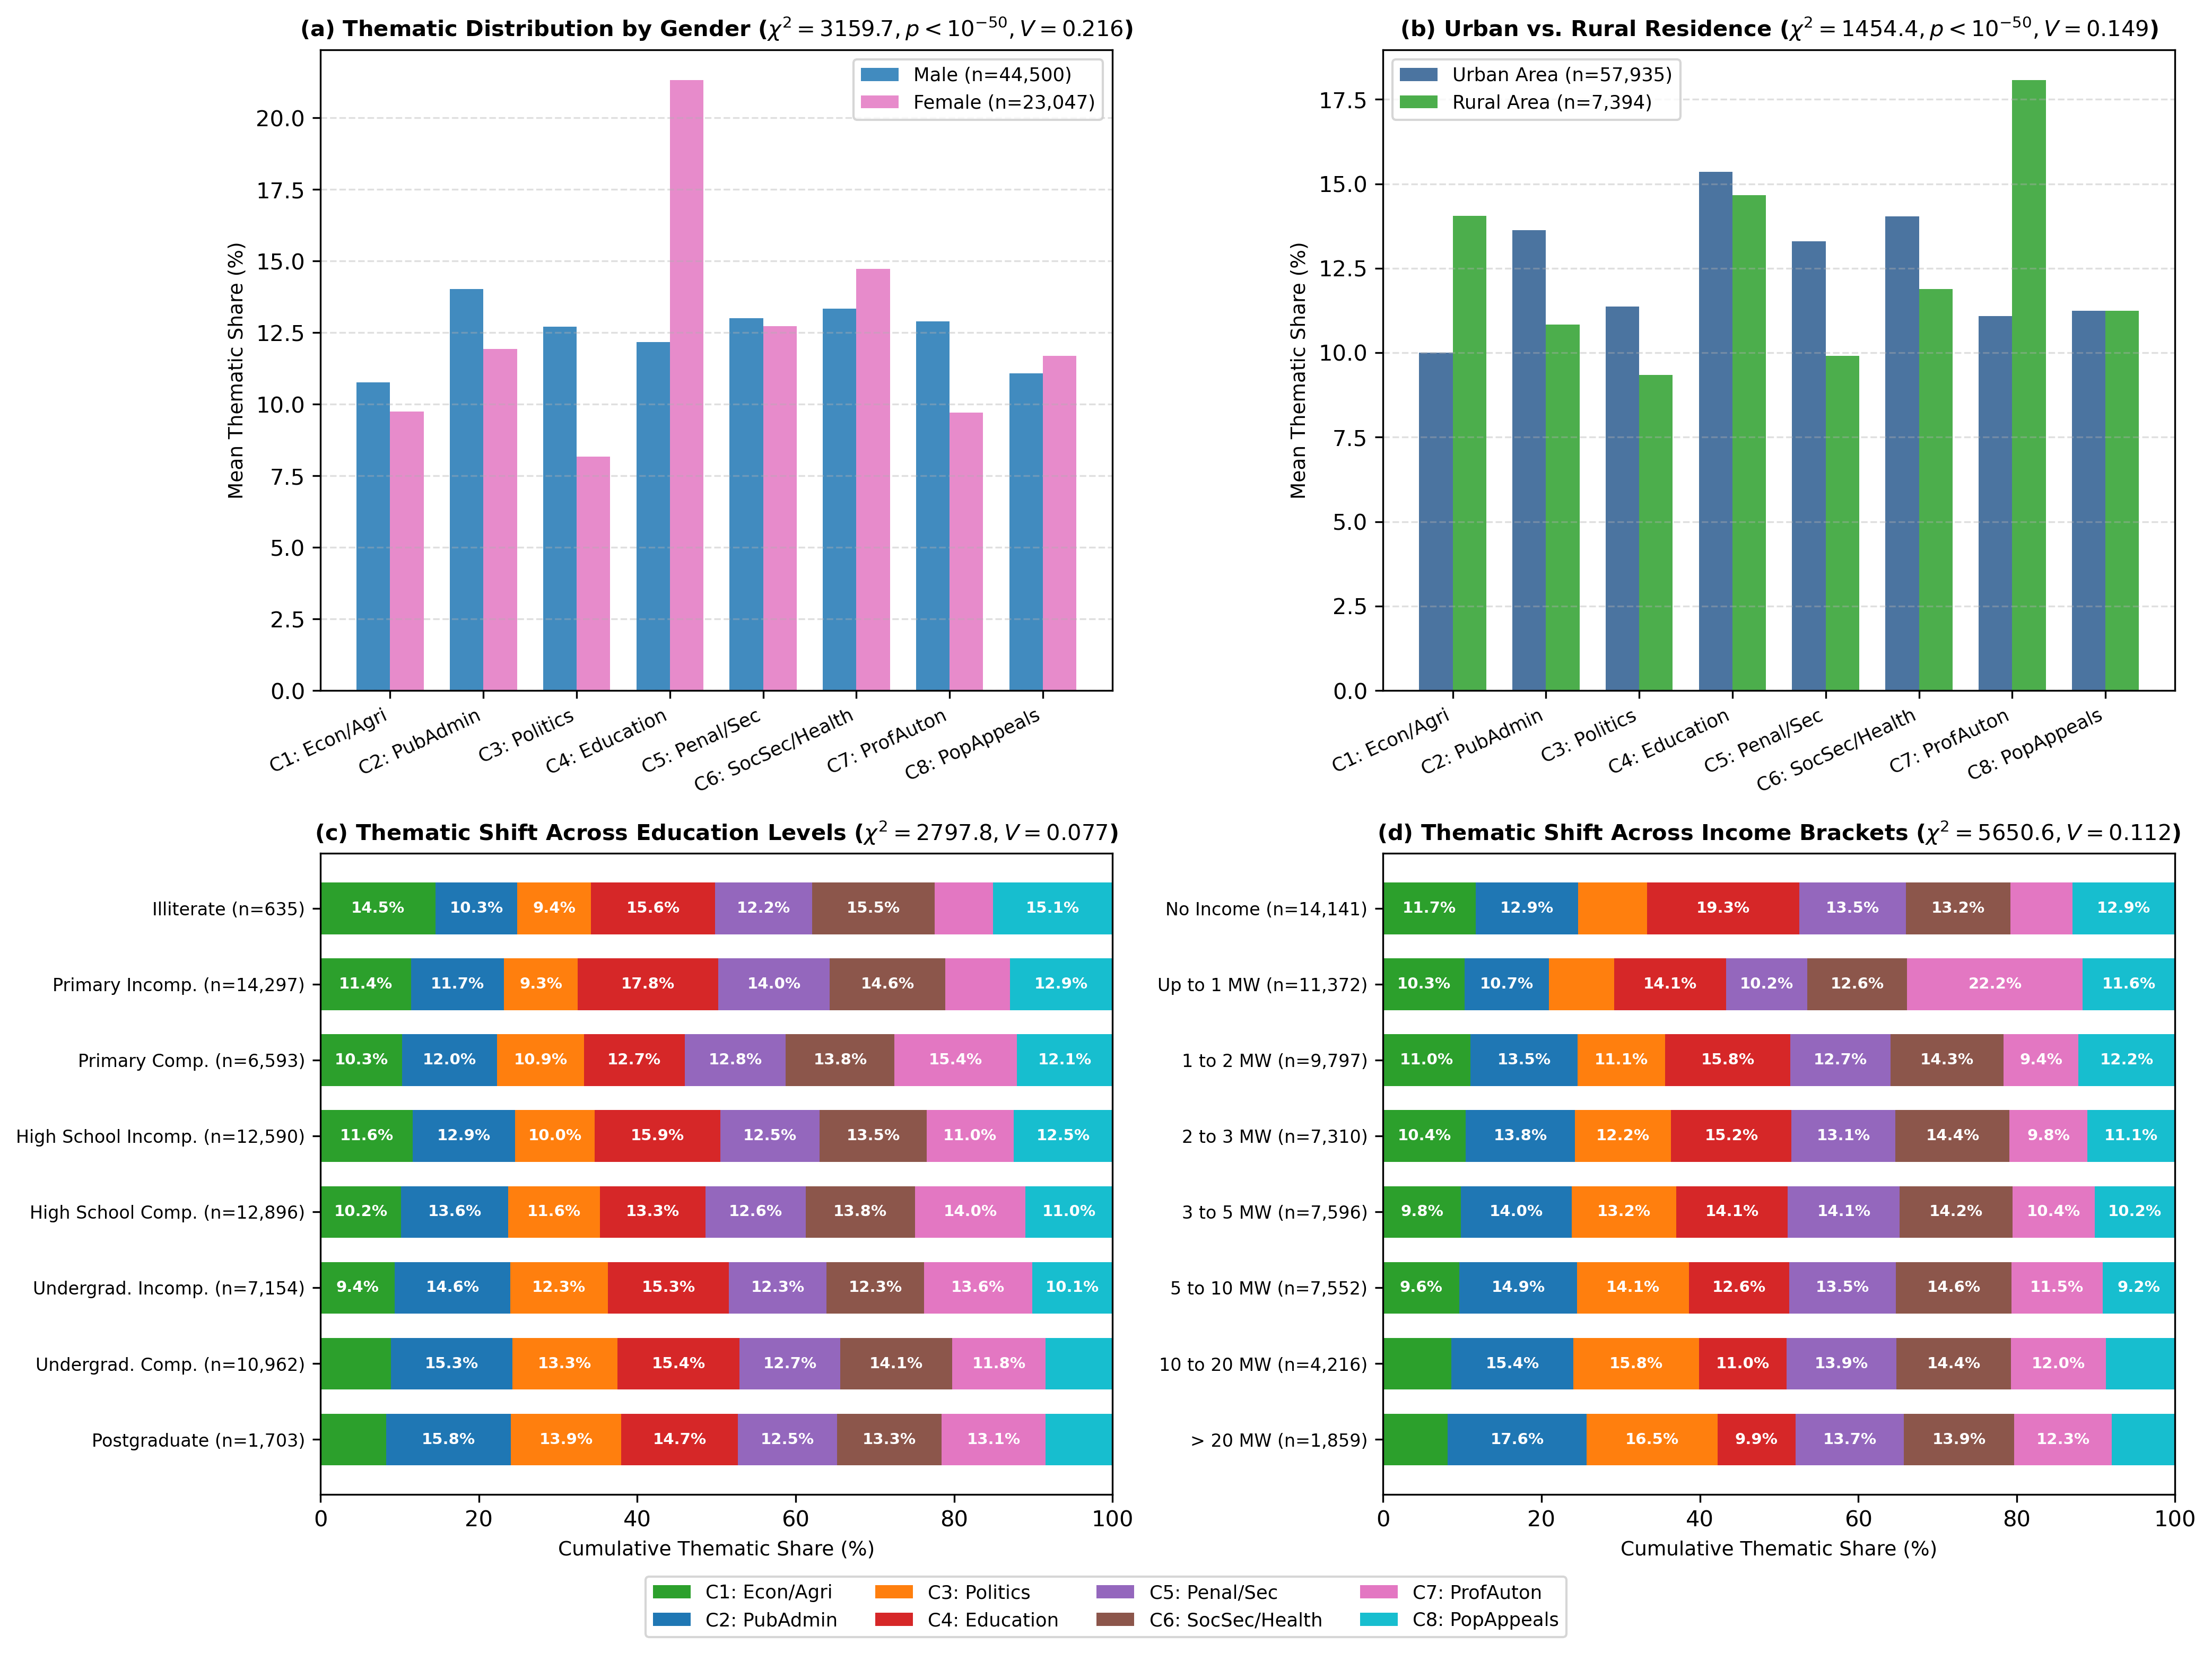
\includegraphics[width=\textwidth]{figures/fig3_demographic_profiles_en.png}
\caption{Thematic stratification and diverging cleavages: (a--c) Grouped mean thematic shares across Gender ($N=67,547$), Urban vs.\ Rural Residence ($N=65,329$), and Mobilization Mode ($N=71,428$); (d--f) Corresponding diverging percentage-point difference ($\Delta$ pp) dot plots highlighting the net directional cleavages.}
\label{fig:demographics}
\end{figure*}

\begin{figure*}[t]
\centering
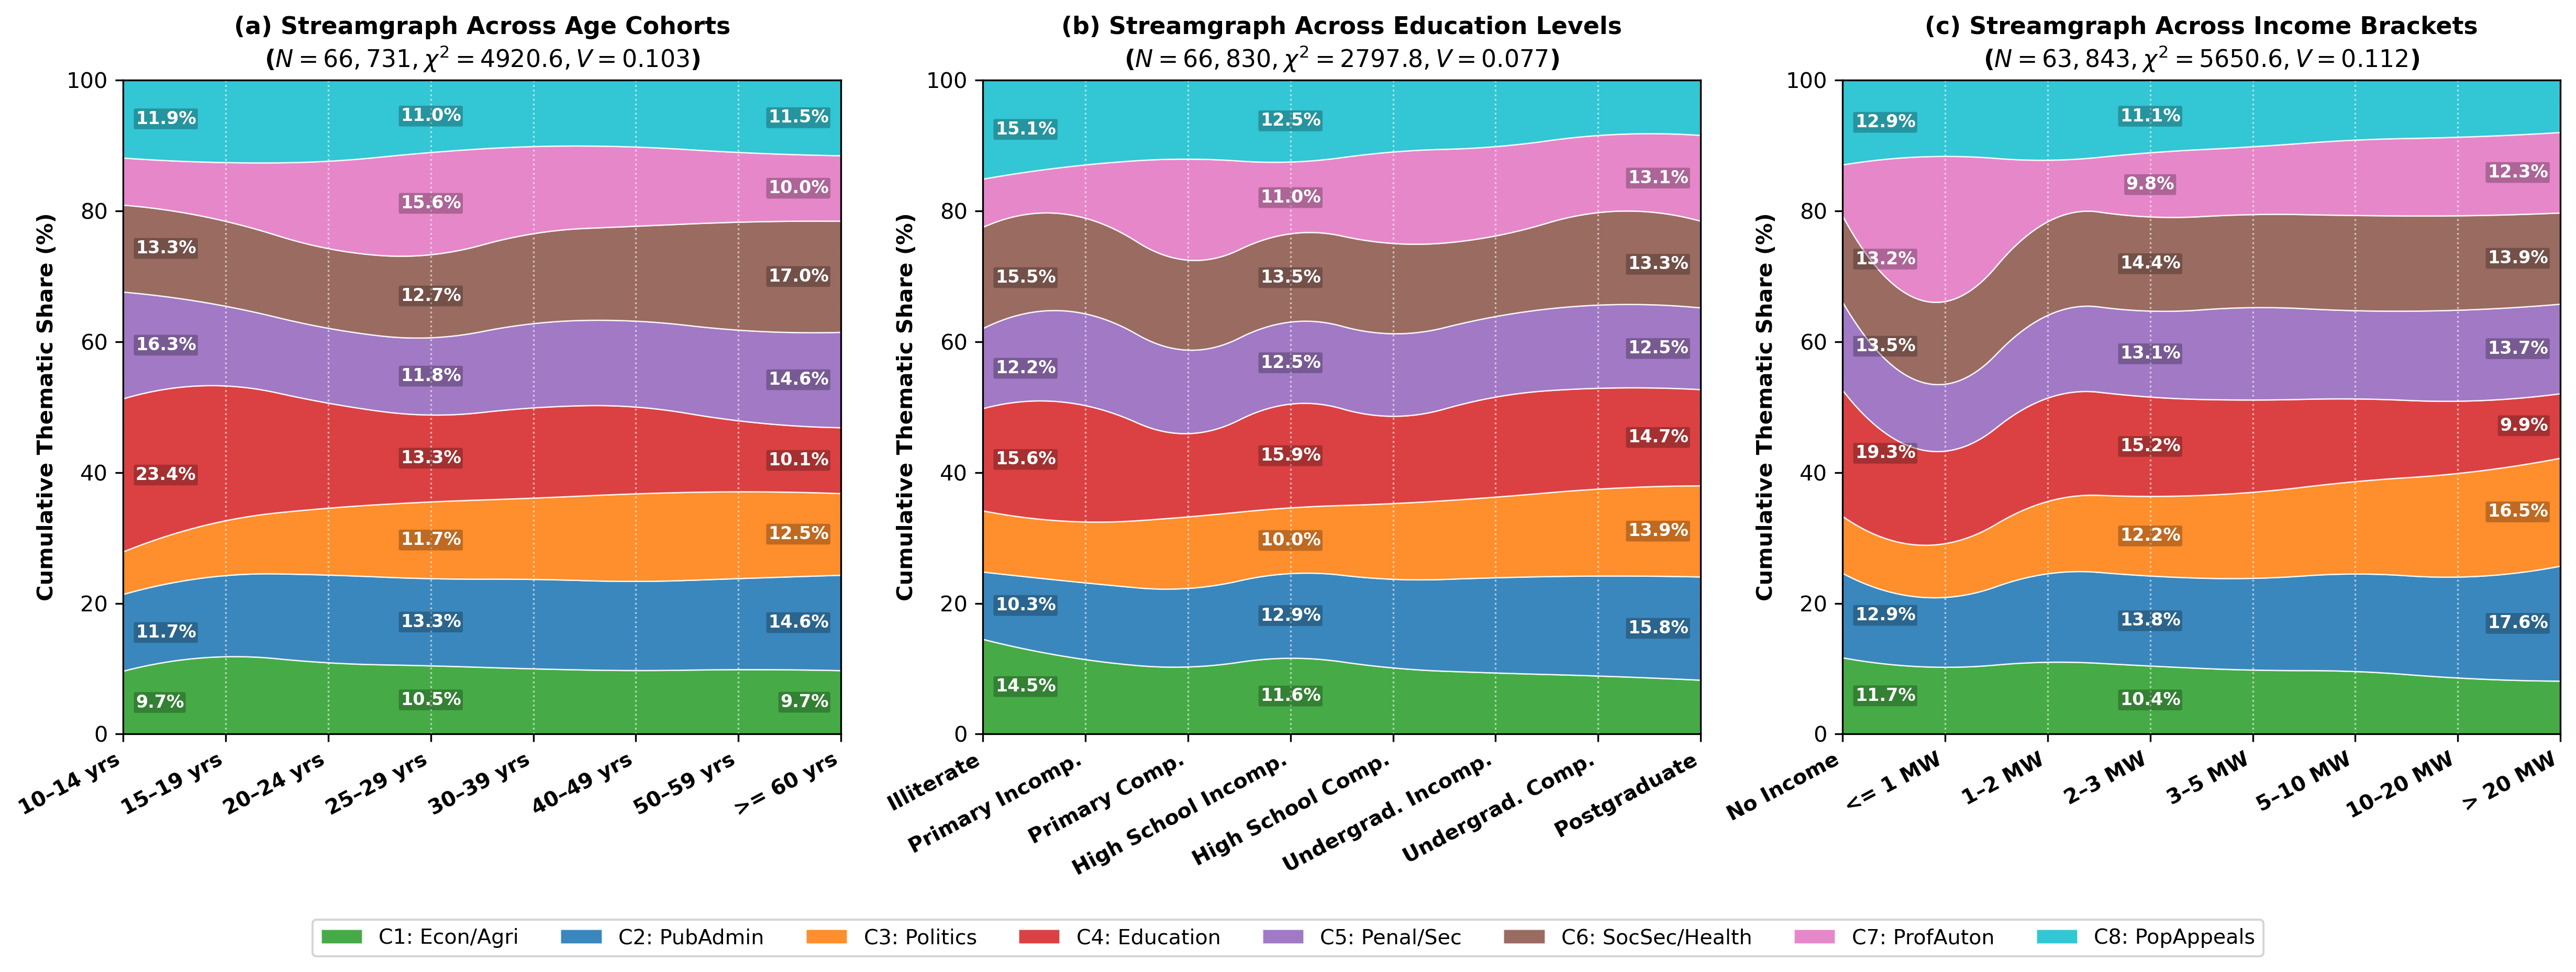
\includegraphics[width=\textwidth]{figures/fig4_streamgraphs_socioeconomic_en.png}
\caption{Continuous cubic-spline streamgraphs of constitutional discourse communities across ordinal life-course and socioeconomic strata: (a) Age Cohorts ($N=66,731$), (b) Educational Attainment Levels ($N=66,830$), and (c) Family Income Brackets in Minimum Wages ($N=63,843$).}
\label{fig:streamgraphs}
\end{figure*}

\subsection{RQ4: Macro-Regional, State-Level Choropleth, and Bipartite Parliamentarian Targeting}
To examine spatial heterogeneity at both macro and sub-national scales, Figure~\ref{fig:choropleth} maps the state-level participation volume ($\log_{10}$ scale) and the dominant constitutional community across all 26 Brazilian states and territories existing in 1986--1987, while Figure~\ref{fig:regional} pairs the full thematic distribution across the five macro-regions ($N=71,310$, $\chi^2 = 5,009.6, p < 10^{-100}, V = 0.133$) with the top 12 federative units ($N=61,218$, $\chi^2 = 8,611.5, p < 10^{-100}, V = 0.142$). The choropleth map (Figure~\ref{fig:choropleth}b) uncovers five striking contiguous geographic belts:
\begin{itemize}
    \item \textbf{The Southern and Center-Western Educational Belt ($C_4$):} A contiguous block spanning \textbf{Rio Grande do Sul (RS, $16\%$)}, \textbf{Santa Catarina (SC, $18\%$)}, \textbf{Paran\'{a} (PR, $31.2\%$)}, \textbf{Mato Grosso do Sul (MS, $18\%$)}, \textbf{Mato Grosso (MT, $18\%$)}, and \textbf{Goi\'{a}s (GO, $27.7\%$)} (plus \textbf{AC} and \textbf{AP}) had \textbf{$C_4$: Educational Policy} as its dominant community, a pattern consistent with intense regional mobilization over public and community school funding.
    \item \textbf{The Southeastern Industrial Welfare and Security Core ($C_6$ and $C_5$):} The most populous states---\textbf{S\~{a}o Paulo (SP, $n=14,739$, $16.3\%$)} and \textbf{Minas Gerais (MG, $n=10,973$, $15.1\%$)} (along with \textbf{PE}, $14.8\%$)---were dominated by \textbf{$C_6$: Social Security \& Healthcare}, whereas coastal metropolitan states \textbf{Rio de Janeiro (RJ, $15.4\%$)} and \textbf{Esp\'{\i}rito Santo (ES, $14.9\%$)} were dominated by \textbf{$C_5$: Penal System \& Public Security}.
    \item \textbf{The Northern--Northeastern Corporatist Belt ($C_7$):} A contiguous corridor across \textbf{Maranh\~{a}o (MA, $15.2\%$)}, \textbf{Piau\'{\i} (PI, $34.3\%$)}, \textbf{Cear\'{a} (CE, $43.6\%$)}, \textbf{Rio Grande do Norte (RN, $22.1\%$)}, and \textbf{Para\'{\i}ba (PB, $26.6\%$)} was heavily dominated by \textbf{$C_7$: Professional Autonomy \& Labor}, while \textbf{Bahia (BA, $14.9\%$)} led in \textbf{$C_3$: Political \& Electoral Structure}.
    \item \textbf{The Amazonian and Federal Administrative Belt ($C_2$):} Across the Amazon basin---\textbf{Amazonas (AM, $15.1\%$)}, \textbf{Par\'{a} (PA, $15.0\%$)}, \textbf{Rond\^{o}nia (RO, $16.1\%$)}, and \textbf{Roraima (RR, $15.4\%$)}---as well as the federal capital \textbf{Distrito Federal (DF, $14.7\%$)}, \textbf{Alagoas (AL, $14.9\%$)}, and \textbf{Sergipe (SE, $14.7\%$)}, citizens prioritized \textbf{$C_2$: Public Administration \& State Organization}, reflecting civil service and federal resource distribution demands.
\end{itemize}

\begin{figure*}[t]
\centering
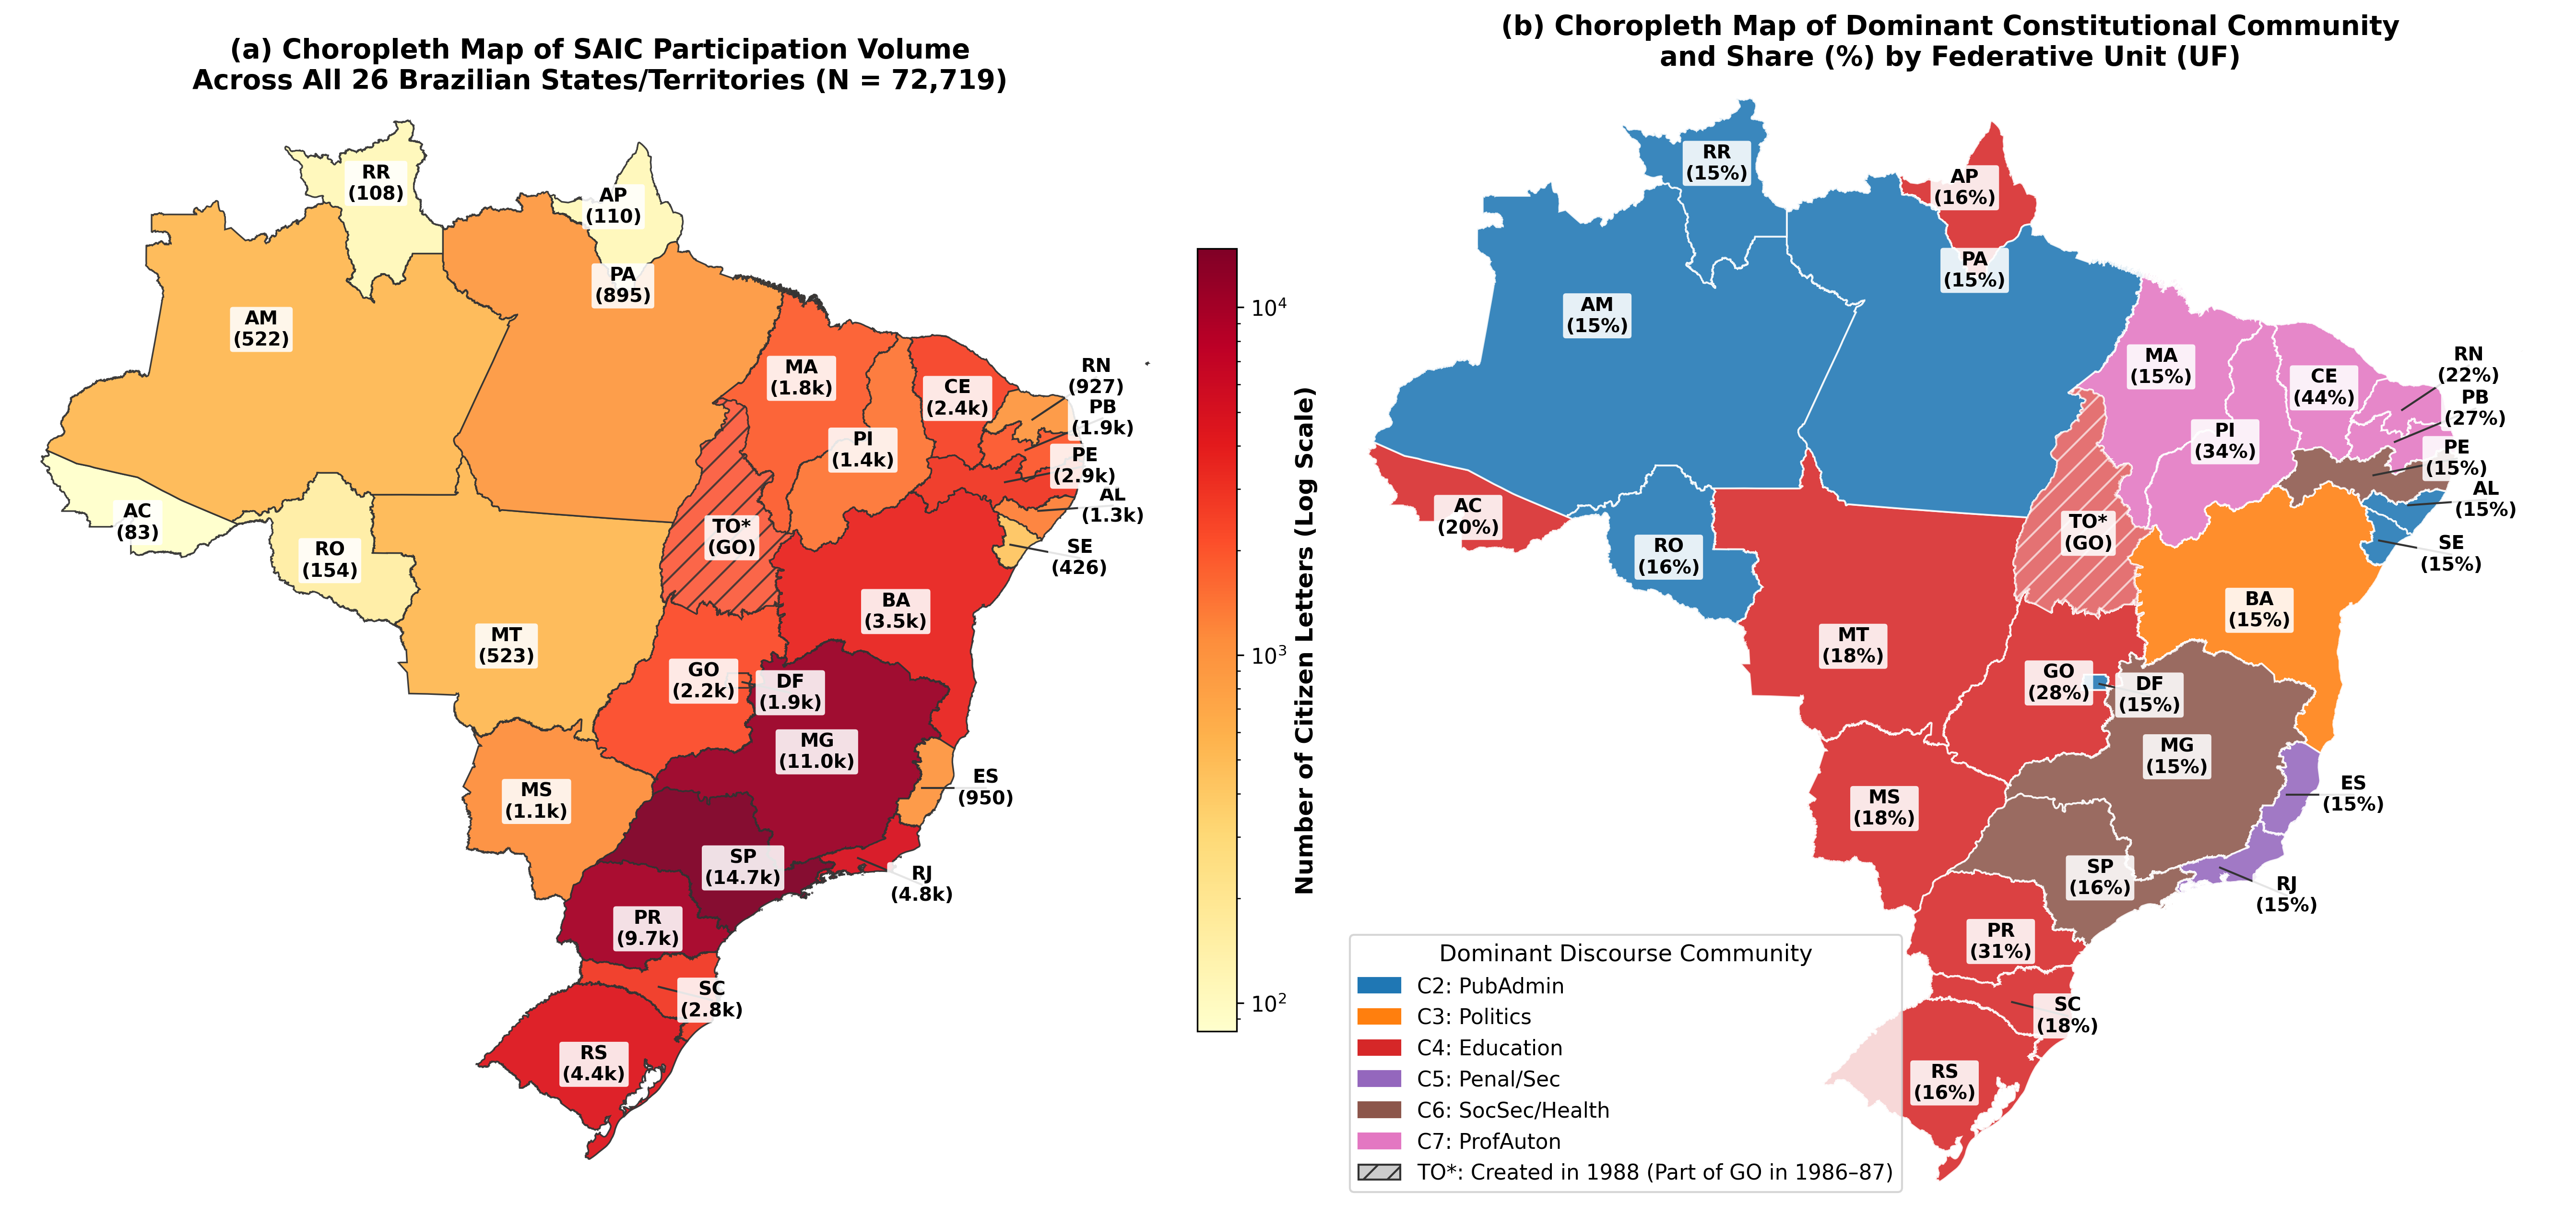
\includegraphics[width=\textwidth]{figures/fig5_choropleth_brazil_en.png}
\caption{State-level choropleth maps of Brazil across all 26 historical Federative Units: (a) Participation volume ($\log_{10}$ scale of citizen letters per UF, $N=72,719$); (b) Dominant constitutional discourse community $c^*(u)$ and its thematic share (\%) per state. Hatched polygon (\texttt{TO*}) denotes the territory of Tocantins, which was part of Goi\'{a}s (\texttt{GO}) during the 1986--1987 SAIC consultation prior to its creation by the 1988 Constitution.}
\label{fig:choropleth}
\end{figure*}

\begin{figure*}[t]
\centering
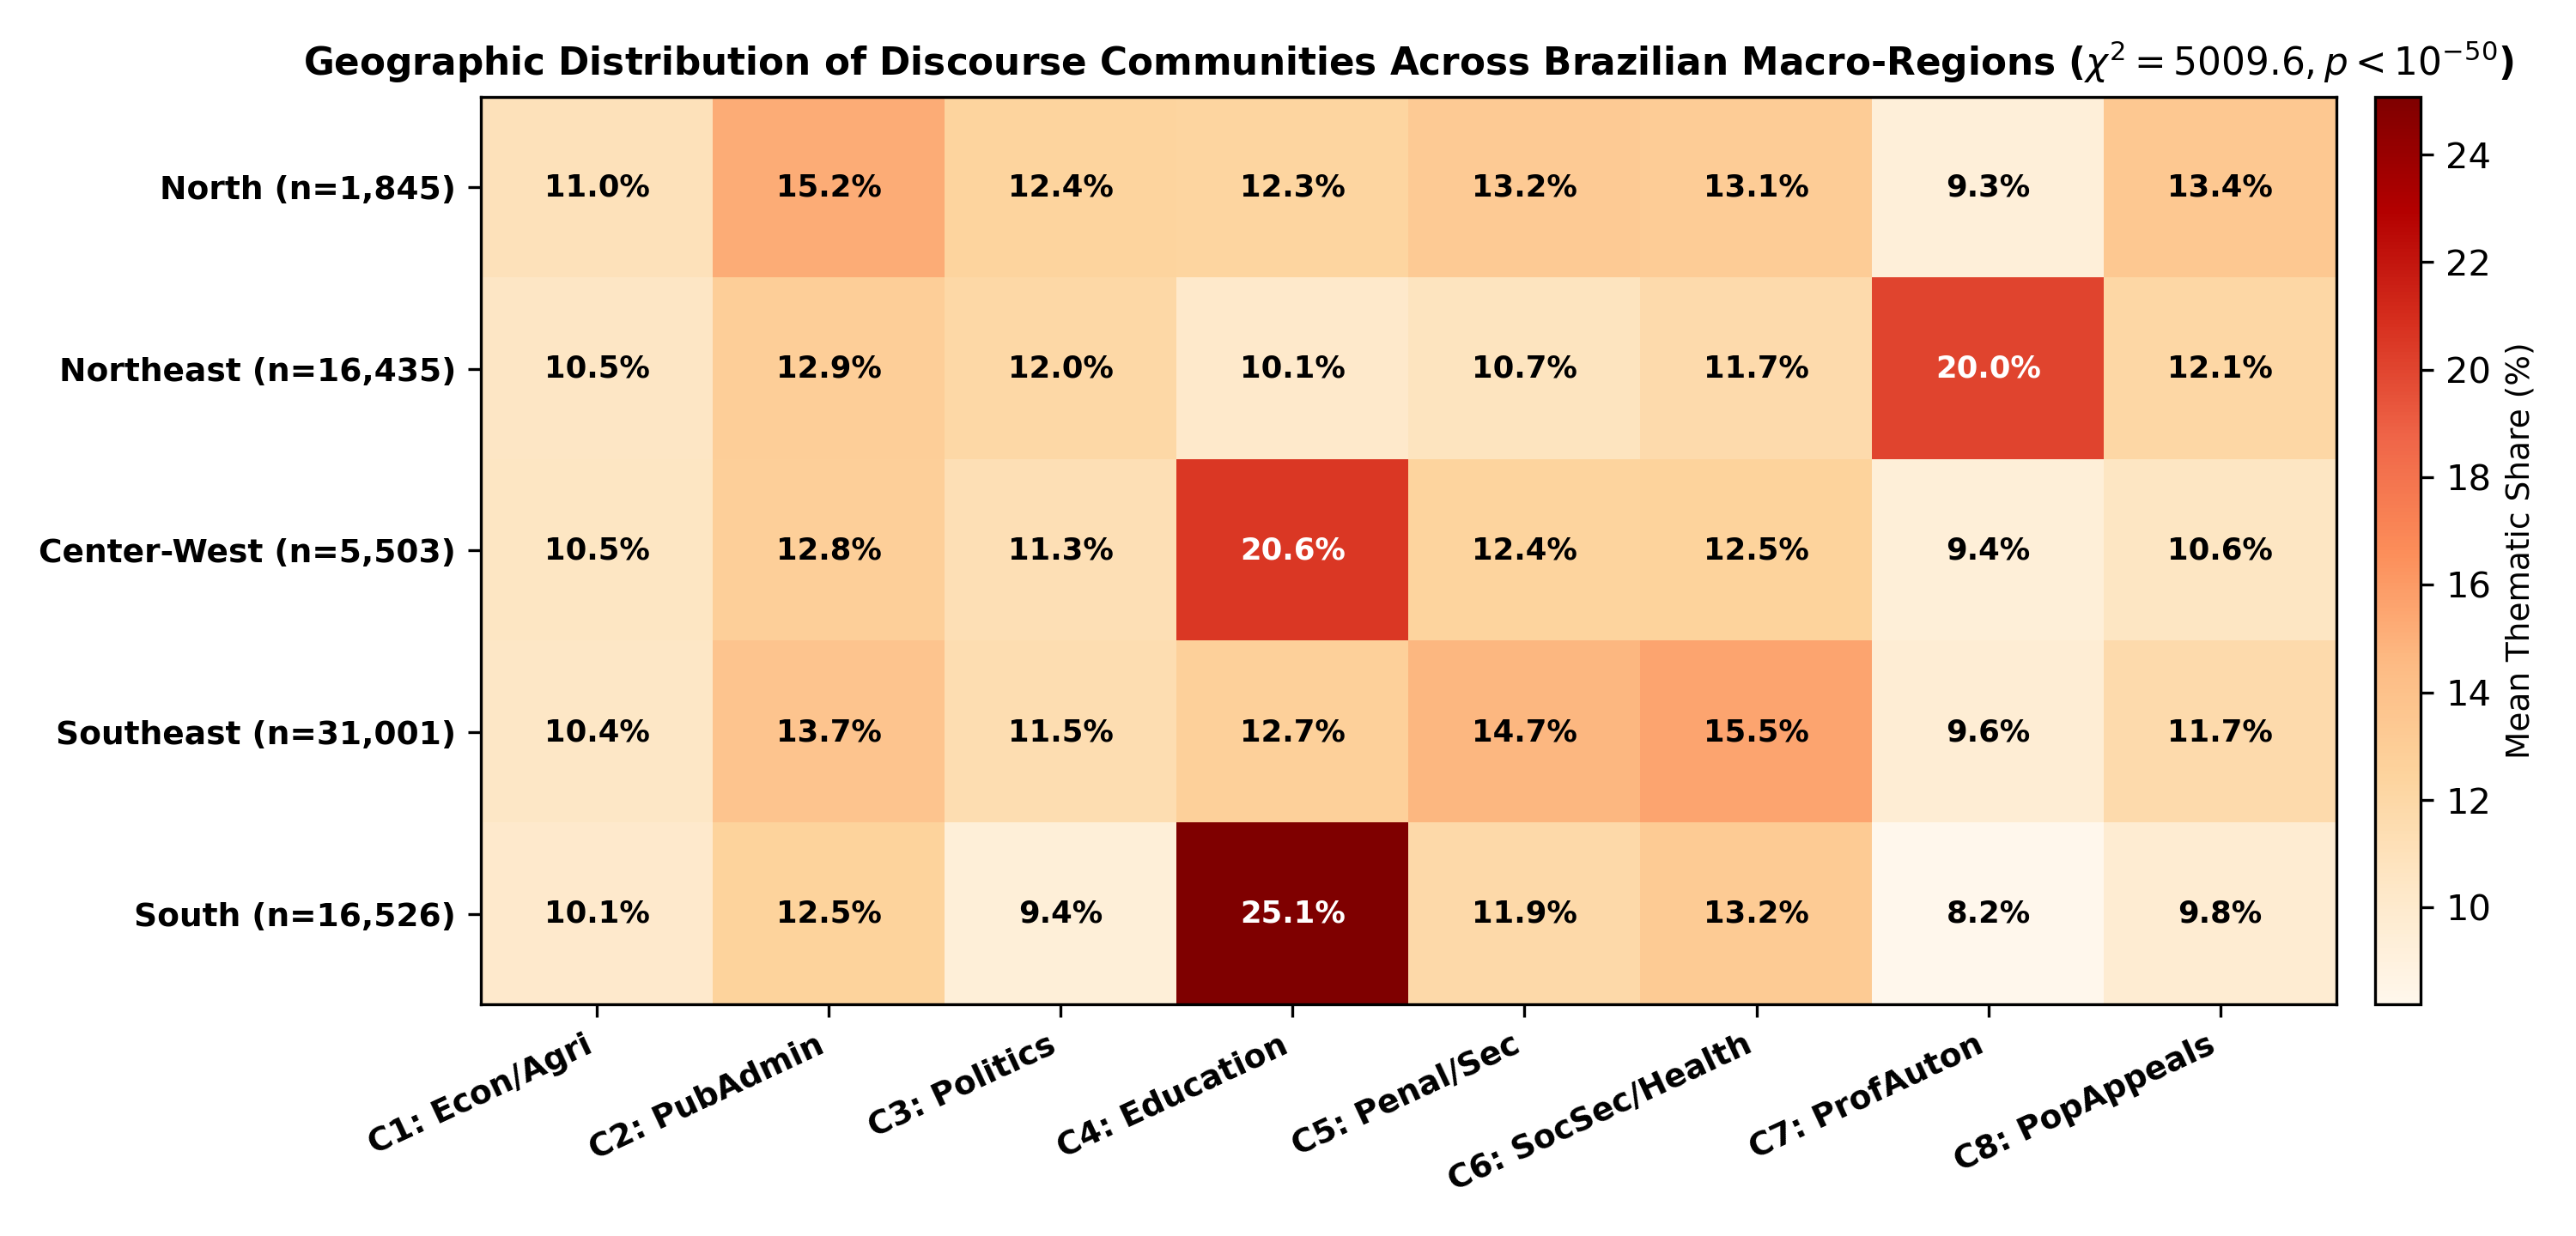
\includegraphics[width=\textwidth]{figures/fig4_regional_distribution_en.png}
\caption{Geographic distribution of constitutional discourse communities across (a) the five Brazilian macro-regions ($N=71,310, \chi^2 = 5,009.6$) and (b) the top 12 Federative Units/States ($N=61,218, \chi^2 = 8,611.5$).}
\label{fig:regional}
\end{figure*}

Finally, we examined the directed targeting of constitutional demands toward the $519$ explicitly named Constituent Assembly members (\texttt{DESTINAT\'{A}RIO}, $N=24,532$ directed letters). To avoid visual clutter and misleading edge density common to bipartite network projections, Figure~\ref{fig:bipartite} displays the cluster-ordered thematic specialization matrix of the top 15 most targeted parliamentarians. Lawmakers are grouped by their dominant community cluster, and horizontal dividers separate specialized functional domains. Rather than receiving a uniform cross-section of public opinion, key lawmakers acted as specialized hubs for distinct social movements:
\begin{enumerate}
    \item \textbf{Presidential and Legislative Leadership Targeted by Corporatist Campaigns ($C_7$):} Senate President \textbf{Humberto Lucena} ($n=576$), ANC President \textbf{Ulysses Guimar\~{a}es} ($n=3,260$), and Senator \textbf{Nelson Carneiro} ($n=963$) received $65.5\%$, $39.9\%$, and $38.3\%$ of their directed letters from $C_7$ (Professional Autonomy \& Labor), reflecting coordinated national lobbying directed at institutional gatekeepers.
    \item \textbf{Educational Policy Champions ($C_4$):} Constituents \textbf{Freitas Nobre} ($n=401$) and \textbf{Jos\'{e} Richa} ($n=265$) were overwhelmingly targeted by educational campaigns, with $61.2\%$ and $44.0\%$ of their correspondence concentrated in $C_4$.
    \item \textbf{Social Welfare, Healthcare, and Public Security Mediators ($C_6$, $C_5$, and $C_2$):} Prominent senators and party leaders---including \textbf{Paulo Maluf} ($n=433$, $17.0\%$), \textbf{Jamil Haddad} ($n=501$, $16.6\%$), \textbf{\'{A}lvaro Dias} ($n=739$, $16.2\%$), \textbf{Carlos Chiarelli} ($n=341$, $16.0\%$), \textbf{Itamar Franco} ($n=498$, $16.0\%$), \textbf{Fernando Henrique Cardoso} ($n=861$, $15.7\%$), \textbf{Alfredo Campos} ($n=392$, $15.6\%$), and \textbf{Pimenta da Veiga} ($n=662$, $14.5\%$)---were predominantly petitioned regarding \textbf{$C_6$: Social Security \& Healthcare}. In contrast, Majority Leader \textbf{M\'{a}rio Covas} ($n=332$) peaked in \textbf{$C_5$: Penal System \& Public Security} ($16.1\%$), and Senate Leader \textbf{Jos\'{e} Fragelli} ($n=291$) peaked in \textbf{$C_2$: Public Administration} ($14.9\%$).
\end{enumerate}

\begin{figure*}[t]
\centering
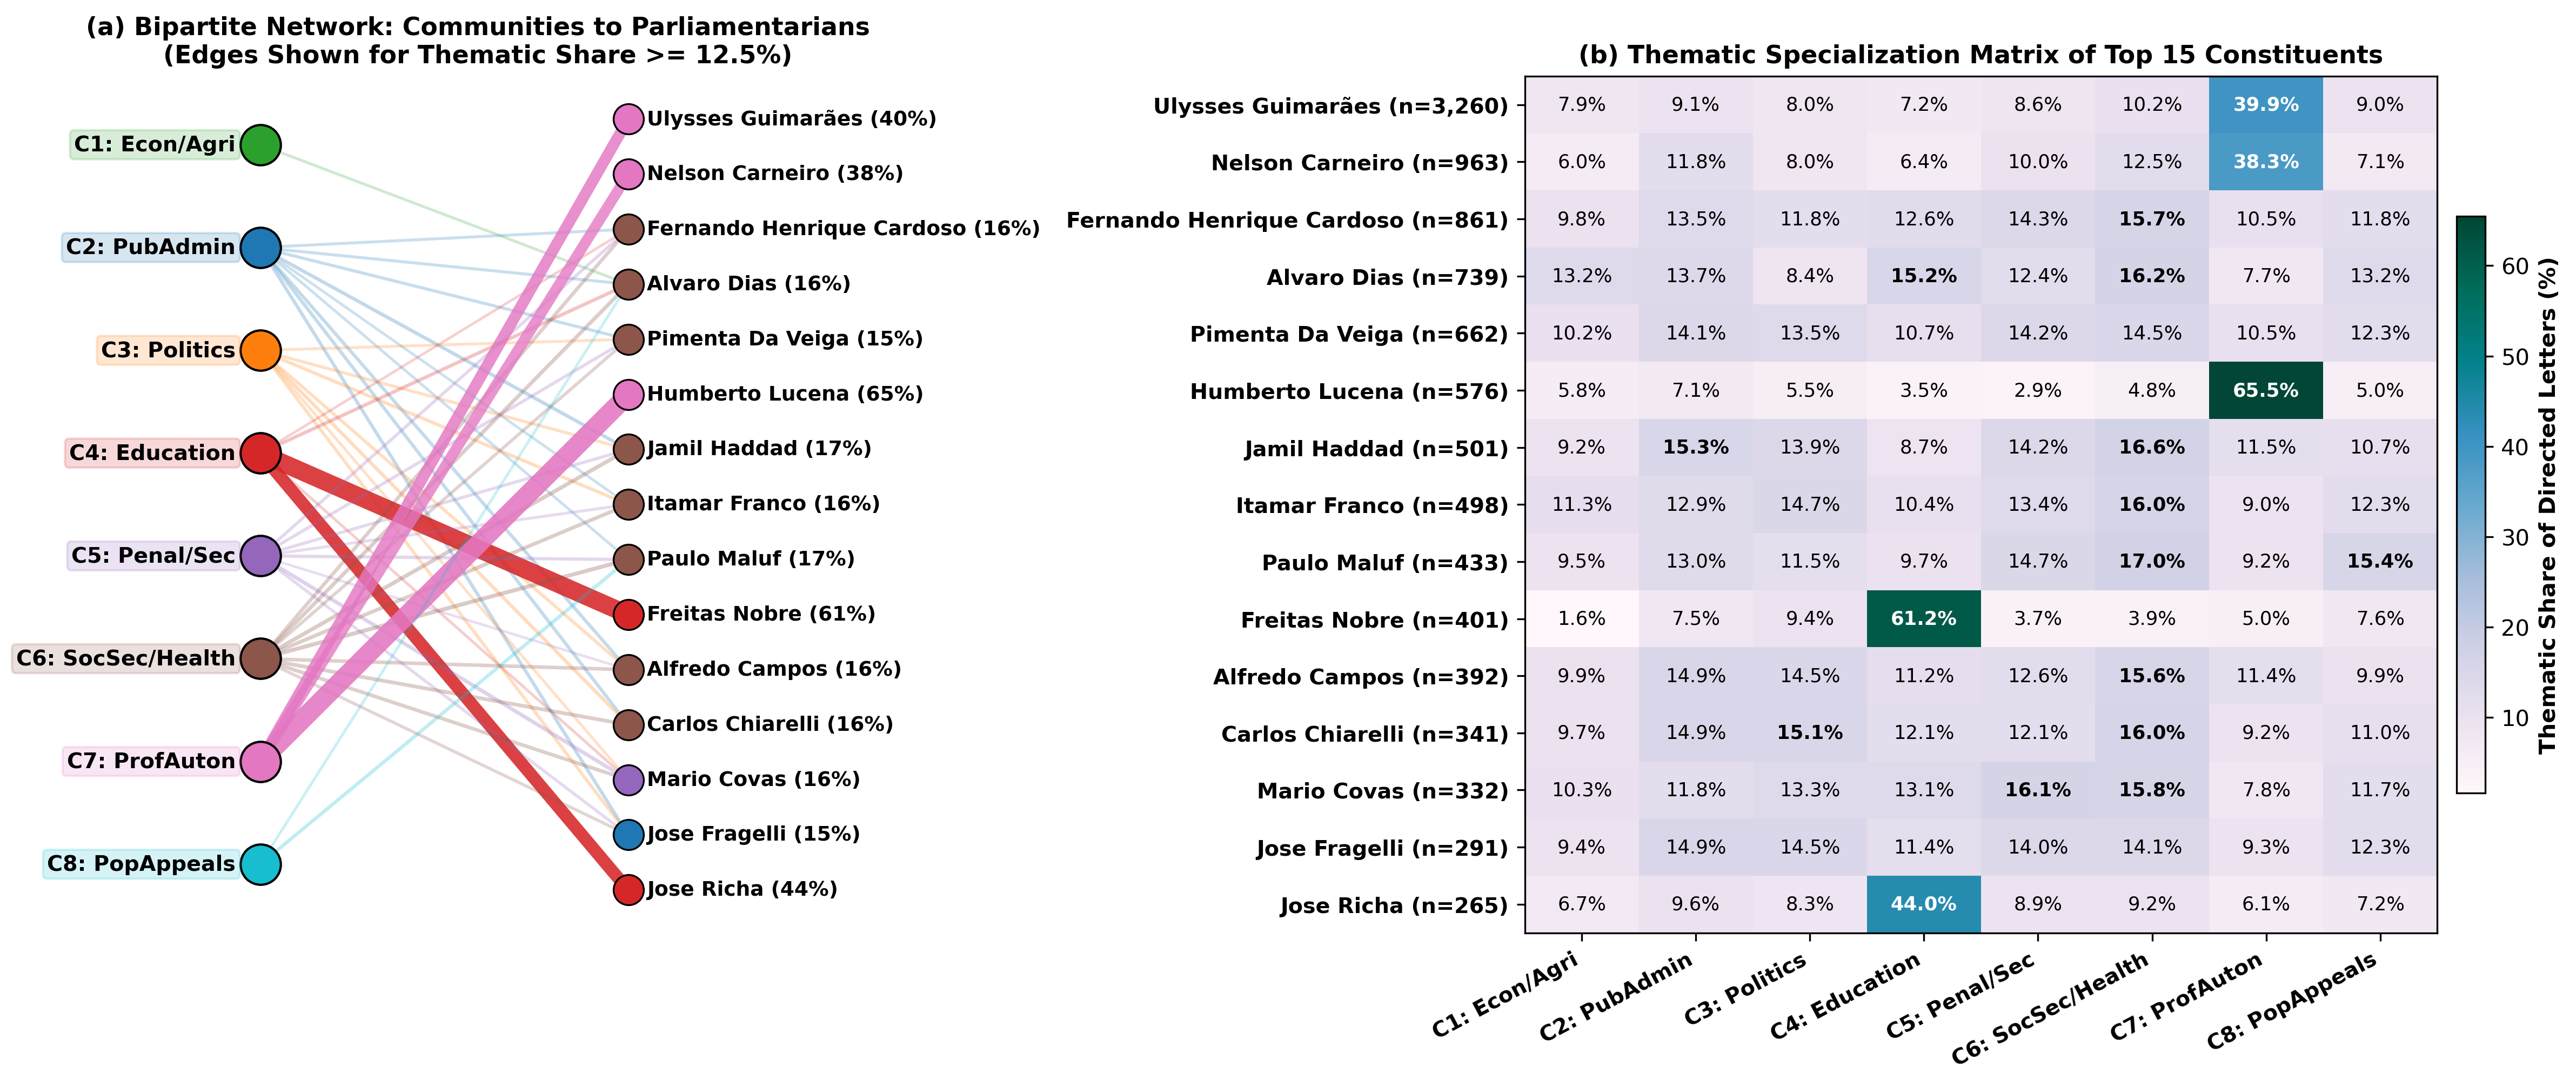
\includegraphics[width=\textwidth]{figures/fig5_bipartite_parliamentarians_en.png}
\caption{Cluster-ordered thematic specialization matrix (\%) of the top 15 targeted Constituent Assembly members in the Citizen--Parliamentarian bipartite network (\texttt{DESTINAT\'{A}RIO}, $N=24,532$). Parliamentarians are sorted by their primary discourse community cluster, with horizontal dividers separating distinct institutional and policy domains.}
\label{fig:bipartite}
\end{figure*}

% [NOVO] Subseção de Limitações
\subsection{Limitations}\label{sec:limitations}
Our design has four limitations that bound the interpretation of the findings. First, the analysis is \emph{descriptive and exploratory}: the strong associations between sociodemographic attributes and thematic communities documented in Section~\ref{sec4} should not be read as causal effects. The SAIC archive records self-selected participants, and unobserved confounders (e.g., local mobilization networks, literacy, access to post offices) plausibly shape both who wrote and what they wrote. Second, the chi-square tests assume independent observations, whereas the corpus contains residual dependence structures beyond the exact duplicates we removed: letters sharing a municipality, an occupation, or a coordinated campaign template are not statistically independent. The reported $p$-values should therefore be read as descriptive indicators of association strength rather than as exact inferential probabilities; Cram\'{e}r's $V$ provides the effect-size counterpart that is robust to sample size. Third, the semantic network is built on document-level co-occurrence, which captures thematic association rather than syntactic or pragmatic structure; a sliding-window formulation would yield a different, more local network. Fourth, community assignments discretize a continuous thematic profile: as noted in Section~3.4, the continuous shares $s_{d,k}$ are the primary quantity, and the dominant-community discretization used for significance testing necessarily discards mixed-membership information.

\section{Conclusion}\label{sec5}
This work presented the first comprehensive complex network and multi-dimensional sociodemographic investigation of the complete 72,719-letter SAIC database from the 1988 Brazilian National Constituent Assembly. By auditing historical data-entry noise (\texttt{\#NOME?}), modeling lexical associations via Positive Pointwise Mutual Information ($\text{min\_df}=2.0\%$, 95th percentile cutoff), and applying Louvain community detection, we extracted a highly modular semantic network ($Q=0.6363$) comprising eight interpretable constitutional discourse communities.

Cross-tabulating these emergent bottom-up communities against Prodasen's 1986 official catalog demonstrated that while unsupervised network clustering aligns closely with specialized administrative labels, it successfully unpacks massive bureaucratic catch-all categories (\textit{Social Organization} and \textit{Law -- State Organization}) into distinct substantive debates. % [ALTERADO] Escopo explícito na conclusão
We emphasize that this contribution is descriptive: the network partition disambiguates certain catch-all categories and exposes cross-cutting debates, but it does not uniformly outperform the official taxonomy, and it also merges administratively distinct themes (e.g., Agricultural and Industrial Policy in $C_1$). Moreover, statistical stratification and continuous streamgraphs across gender, urban/rural residence, spontaneous vs.\ coordinated campaigns, age cohorts, schooling, income, macro-regions, states, and targeted parliamentarians revealed profound structural cleavages in how different segments of Brazilian society envisioned the democratic social contract: women, youth, and Southern/Center-Western citizens (especially in Paran\'{a} and Goi\'{a}s) acted as the primary vanguards for public education ($C_4$); rural and lower-income workers mobilized around land, agricultural credit, and labor autonomy ($C_1, C_7$); urban, older, and Southeastern citizens demanded social security, healthcare, and public safety ($C_6, C_5$); and higher-income, highly educated strata dominated discussions on fiscal federalism, civil service rules, and electoral engineering ($C_2, C_3$). These patterns are associational rather than causal, and the limitations discussed in Section~\ref{sec:limitations} should be kept in mind when interpreting them.

Future research will extend this open-science repository by incorporating contextualized embeddings \citep{amancio2025leveraging} to track how specific grassroots clusters directly influenced the final articles promulgated in the 1988 Federal Constitution.

\section*{Declarations}
\noindent\textbf{Funding:} The authors received no specific funding for this work.\\[3pt]
\noindent\textbf{Competing Interests:} The authors declare that they have no competing interests.\\[3pt]
\noindent\textbf{Compliance with Ethical Standards:} This study analyzes a publicly accessible historical mainframe dataset released by the Federal Senate of Brazil. No human subjects were actively recruited or subjected to experimental interventions.\\[3pt]
\noindent\textbf{Data and Code Availability:} In compliance with Open Science standards, the curated dataset, high-resolution figures, and an interactive Google Colab replication notebook are publicly available at \url{https://github.com/alkawamo/snam-saic-1988} and \url{https://github.com/alkawamo/base-saic}.\\[3pt]
\noindent\textbf{Authors' Contributions:} R.R.M. curated the dataset, implemented the network modeling pipeline, and wrote the initial draft. A.L.S.K. conceptualized the study, designed the multi-dimensional stratification framework, supervised the project, performed the statistical analyses, and reviewed the manuscript. Both authors read and approved the final manuscript.

\bibliography{references}

\end{document}